\chapter{Solución Propuesta}

\section{Propuesta de Solución}
Se elaboró un sistema de realidad virtual del sistema digestivo del cuerpo humano que permite interactuar con modelos tridimensionales.
 La intención es sentar las bases para un sistema de apoyo al aprendizaje que sea más práctico \cite{moore1995learning}, 
 sin sustituir a ningún método de estudio tradicional.\\

\section{Arquitectura del sistema}
%Diagrama de despliegue
%Que componentyes tiene y se crearon
%ver, interactuar y mover

\section{Viabilidad} \label{viab}
También se analizó la factibilidad del proyecto en general. Desde el punto de vista técnico se realizó una evaluación de la tecnología 
actual existente y la posibilidad de utilizarla en el desarrollo del sistema. Además de DirectX versión 11 el cuadro \ref{tab:t23} 
muestra los recursos técnicos necesarios para la ejecución correcta del software:\\
\begin{table}[H]
\centering
\begin{tabular}{|c|c|l|}
\hline
\rowcolor[HTML]{9B9B9B} 
\textbf{Cantidad} &
  \textbf{Recursos} &
  \multicolumn{1}{c|}{\cellcolor[HTML]{9B9B9B}\textbf{Características}} \\ \hline
\cellcolor[HTML]{C0C0C0}1 &
  Computadora Personal de Escritorio &
  \begin{tabular}[c]{@{}l@{}}Tarjeta gráfica discreta, RX480\\ Memoria RAM 16 Gb\\ 5 Puertos USB\\ Procesador de 4 núcleos o mayor\end{tabular} \\ \hline
\cellcolor[HTML]{C0C0C0}1 &
  Sistema de realidad Virtual Oculus Rift &
  \begin{tabular}[c]{@{}l@{}}Visor HMD, controles Touch \\ \\ Sensores Touch.\end{tabular} \\ \hline
\end{tabular}
\caption{ Recursos Técnicos.}
\label{tab:t23}
\end{table}
Económicamente, se determinaron los recursos para desarrollar el sistema así como la comparativa con el uso de cuerpos para su examinación y estudio. Después de un análisis e 
investigación de los costos con la dirección del Área de Morfología en la Escuela Superior de Medicina bajo la asesoría del Dr. Macias Rios se determinó que el costo que se 
tiene para el traslado, mantenimiento, uso e inhumación de los cuerpos es de \$40,000.00 c/u, como se ve en el cuadro \ref{tab:t24}.
\begin{table}[H]
\centering
\begin{tabular}{|
>{\columncolor[HTML]{C0C0C0}}c |l|}
\hline
\multicolumn{2}{|c|}{\cellcolor[HTML]{9B9B9B}\textbf{Costo de uso de cuerpos.}} \\ \hline
Traslado, mantenimiento, uso e inhumación           & \$40,000.00 c/u           \\ \hline
Total                                               & \$40,000.00 c/u           \\ \hline
\end{tabular}
\caption{Costo de cálculo de uso de cuerpos.}
\label{tab:t24}
\end{table}

En el caso del desarrollo e implementación del proyecto se consideró la depreciación, como se observa en el cuadro \ref{tab:t25}.
\begin{table}[H]
\centering
\resizebox{\textwidth}{!}{%
\begin{tabular}{clccccc|c|c|}
\hline
\rowcolor[HTML]{9B9B9B} 
\multicolumn{9}{|c|}{\cellcolor[HTML]{9B9B9B}\textbf{Depreciaciones del Proyecto}} \\ \hline
\rowcolor[HTML]{9B9B9B} 
\multicolumn{4}{|c|}{\cellcolor[HTML]{9B9B9B}\textbf{Equipos de Cómputo}} &
  \multicolumn{5}{c|}{\cellcolor[HTML]{9B9B9B}\textbf{Depreciación}} \\ \hline
\rowcolor[HTML]{9B9B9B} 
\multicolumn{1}{|c|}{\cellcolor[HTML]{9B9B9B}\textbf{Cantidad}} &
  \multicolumn{1}{c|}{\cellcolor[HTML]{9B9B9B}\textbf{Equipos}} &
  \multicolumn{1}{c|}{\cellcolor[HTML]{9B9B9B}\textbf{\begin{tabular}[c]{@{}c@{}}Monto original de \\ Inversión\end{tabular}}} &
  \multicolumn{1}{c|}{\cellcolor[HTML]{9B9B9B}\textbf{\begin{tabular}[c]{@{}c@{}}Valor actual\\  del equipo\end{tabular}}} &
  \multicolumn{1}{c|}{\cellcolor[HTML]{9B9B9B}\textbf{\begin{tabular}[c]{@{}c@{}}Valor a \\ \\ depreciar\end{tabular}}} &
  \multicolumn{1}{c|}{\cellcolor[HTML]{9B9B9B}\textbf{\begin{tabular}[c]{@{}c@{}}\%\\ anual\end{tabular}}} &
  \textbf{\begin{tabular}[c]{@{}c@{}}\%\\ mensual\end{tabular}} &
  \textbf{\begin{tabular}[c]{@{}c@{}}Depresiación\\ mensual\end{tabular}} &
  \textbf{\begin{tabular}[c]{@{}c@{}}Depreciación\\ anual\end{tabular}} \\ \hline
\multicolumn{1}{|c|}{\cellcolor[HTML]{C0C0C0}1} &
  \multicolumn{1}{l|}{\begin{tabular}[c]{@{}l@{}}Computadora de\\ escritorio armada\end{tabular}} &
  \multicolumn{1}{c|}{\$25,054.63} &
  \multicolumn{1}{c|}{\$20,000.00} &
  \multicolumn{1}{c|}{\$5,054.63} &
  \multicolumn{1}{c|}{33.33\%} &
  2.78\% &
  \$ 140.52 &
  \$1,545.72 \\ \hline
\multicolumn{1}{|c|}{\cellcolor[HTML]{C0C0C0}1} &
  \multicolumn{1}{l|}{Laptop HP} &
  \multicolumn{1}{c|}{\$9,999.00} &
  \multicolumn{1}{c|}{\$6,999.00} &
  \multicolumn{1}{c|}{\$3,000.00} &
  \multicolumn{1}{c|}{33.33\%} &
  2.78\% &
  \$ 83.40 &
  \$ 917.40 \\ \hline
\multicolumn{7}{l}{} &
  \textbf{Total:} &
  \$ 2,463.12 \\ \cline{8-9} 
\end{tabular}
}
\caption{Depreciaciones del proyecto.}
\label{tab:t25}
\end{table}

Para ofrecer una experiencia aceptable al momento del uso del equipo de Realidad Virtual 
y el software se proponen los elementos del cuadro \ref{tab:componentes}. La computadora 
que se armó tuvo un costo aproximado de \$25,000.00 MXN, ya considerando los demás componentes.

\begin{table}
\centering
\begin{tabular}{|c|c|}\hline
{\bf Componente} & {\bf Modelo}\\\hline
Procesador & AMD Ryzen 5 1600, 3.20GHz\\\hline
Memoria RAM & 16 Gio DDR4\\\hline
Tarjeta de Video & AMD Radeon RX 480 8Gio\\\hline
\end{tabular}
\caption{Componentes principales de la computadora armada que se usó para el proyecto.}
\label{tab:componentes}
\end{table}

\textbf{Pendiente tabla costos}\\
Además, el sistema de Realidad Virtual con sus componentes tiene un costo que se muestra en el cuadro \ref{tab:t27}.
\begin{table}[H]
  \centering
  \begin{tabular}{|c|c|}
  \hline
  \rowcolor[HTML]{9B9B9B} 
  \multicolumn{2}{|c|}{\cellcolor[HTML]{9B9B9B}\textbf{Sistema de Realidad Virtual}} \\ \hline
  \rowcolor[HTML]{9B9B9B} 
  \textbf{Producto}                          & \textbf{Producto}                     \\ \hline
  Visor Oculus Rift                          & Incluido en el paquete                \\ \hline
  Controles Touch Oculus x 2                 & Incluido en el paquete                \\ \hline
  Sensores Oculus x 2                        & Incluido en el paquete                \\ \hline
  Anexos                                     & Incluido en el paquete                \\ \hline
  \textbf{Total:}                            & \$ 8,821.74                           \\ \hline
  \end{tabular}
  \caption{Costos y contenido del sistema de Realidad Virtual.}
  \label{tab:t27}
\end{table}

Se estimaron los sueldos de programador y modelado, como se observa en el cuadro \ref{tab:t28}.\\
\begin{table}[H]
  \centering
  \resizebox{\textwidth}{!}{%
  \begin{tabular}{ccc|c|c|}
  \hline
  \rowcolor[HTML]{9B9B9B} 
  \multicolumn{5}{|c|}{\cellcolor[HTML]{9B9B9B}\textbf{Sueldos}}                                                                                                                                                                                                                                                                    \\ \hline
  \rowcolor[HTML]{9B9B9B} 
  \multicolumn{1}{|c|}{\cellcolor[HTML]{9B9B9B}\textbf{Puesto}} & \multicolumn{1}{c|}{\cellcolor[HTML]{9B9B9B}\textbf{\begin{tabular}[c]{@{}c@{}}Sueldo\\ Mensual\\ individual\end{tabular}}} & \textbf{\begin{tabular}[c]{@{}c@{}}Cantidad \\ \\ de personal\end{tabular}} & \textbf{Sueldos mensuales totales} & \textbf{6 meses} \\ \hline
  \multicolumn{1}{|c|}{Programador}                             & \multicolumn{1}{c|}{\$25,296.00}                                                                                            & 1                                                                           & \$25,296.00                        & \$151,776.00     \\ \hline
  \multicolumn{1}{|c|}{Modelador 3D}                            & \multicolumn{1}{c|}{\$25,296.00}                                                                                            & 1                                                                           & \$25,296.00                        & \$151,776.00     \\ \hline
  \multicolumn{3}{l}{}                                                                                                                                                                                                                                                      & \multicolumn{1}{l|}{Total}         & \$303,522.00     \\ \cline{4-5} 
  \end{tabular}%
  }
  \caption{Cálculo de Sueldos.
  }
  \label{tab:t28}
\end{table}

\begin{table}[H]
  \centering
  \begin{tabular}{c|c|c|}
  \hline
  \rowcolor[HTML]{9B9B9B} 
  \multicolumn{3}{|c|}{\cellcolor[HTML]{9B9B9B}\textbf{Servicios}}                                       \\ \hline
  \rowcolor[HTML]{9B9B9B} 
  \multicolumn{1}{|c|}{\cellcolor[HTML]{9B9B9B}\textbf{Concepto}} & \textbf{Mensual} & \textbf{11 Meses} \\ \hline
  \multicolumn{1}{|c|}{Luz (kw Consumidos por costo Unitario)}    & \$430            & \$4,730           \\ \hline
  \multicolumn{1}{|c|}{Agua (Lt consumidos por costo unitario)}   & \$200            & \$2,200           \\ \hline
  \multicolumn{1}{|c|}{Teléfono e Internet (renta mensual fija)}  & \$ 450           & \$4,850           \\ \hline
  \multicolumn{1}{l|}{}                                           & Total:           & \$11,780          \\ \cline{2-3} 
  \end{tabular}
  
  \caption{Cálculo de Costo por Servicios.}
  \label{tab:t29}
\end{table}

Los servicios estimados se muestran en el cuadro \ref{tab:t29} y en el cuadro \ref{tab:t210} se muestra la suma total y como resultado se obtiene el costo total del proyecto, 
que se estima en: \$326,316.86.\\
\begin{table}[H]
  \centering
  \begin{tabular}{|l|r|}
  \hline
  \rowcolor[HTML]{9B9B9B} 
  \multicolumn{2}{|c|}{\cellcolor[HTML]{9B9B9B}\textbf{Costos del Proyecto}}                                                    \\ \hline
  \rowcolor[HTML]{9B9B9B} 
  \multicolumn{1}{|c|}{\cellcolor[HTML]{9B9B9B}\textbf{Concepto}} & \multicolumn{1}{c|}{\cellcolor[HTML]{9B9B9B}\textbf{Costo}} \\ \hline
  Servicios                                                       & \$ 11,780                                                   \\ \hline
  Sueldos                                                         & \$303,522.00                                                \\ \hline
  Depreciaciones                                                  & \$2,463.12                                                  \\ \hline
  Equipo extra.                                                   & \$ 8,821.74                                                 \\ \hline
  Total                                                           & \$ 326,316.86                                               \\ \hline
  \end{tabular}
  \caption{Costos finales del proyecto}
  \label{tab:t210}
  \end{table}

En resumen, el costo de usar nueve cuerpos sería de \$360,000.00 y el del proyecto de \$326,318.00, con lo cual se puede considerar viable económicamente.\\

\section{Requerimientos}

\subsection{Funcionales}

\subsection{No Funcionales}
%Se utiliza oclus
%Equipo con estas caracteristicas

\section{Casos de Uso}
El planteamiento de casos de uso en un sistema no tradicional como este puede generar un dificultades al momento de expresar cuál es la actividad que podrá 
realizar el actor ya que las  pero se pueden denotar en acciones específicas que queremos que el usuario pueda realizar en el sistema.\\
%TODO Imagen de el caso de uso.
Ahora bien en la figura 3 se muestran los casos de uso que dan parte a el uso del software y las posibilidades generales de interacción en un software de 
Realidad Virtual. Aunque las interacciones pueden ser prácticamente infinitas estas se ven limitadas hasta cierto punto por las capacidades integradas dentro 
del software, más adelante se describirán las interacciones con los modelos 3D de los sistemas elegidos, en este caso el sistema de realidad virtual.

\section{Metodología}

%\subsection{OpenUP}
%OpenUP [ 14 ] es un proceso de desarrollo de software basado en RUP, publicado con licencia de código abierto donde solo se incluye el contenido mínimo y fundamental. 
%Se puede utilizar como base de desarrollo en procesos específicos, ya que no posee todos los elementos para un proyecto de gran tamaño. Debido a lo anterior OpenUP 
%es extensible de tal manera que puede ser utilizado como base, donde se puede adaptar o añadir el contenido necesario para desarrollar un proyecto.\\
%\begin{figure}[H]
%	\begin{center}
% 		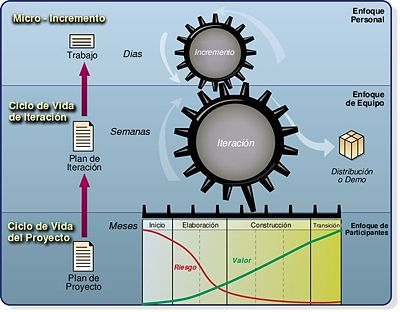
\includegraphics[width = 1\textwidth]{v2/images/image47.png}
% 		\captionof{figure}{\label{fig:me2}Ciclo de Vida Iterativo de OpenUP}
%	\end{center} 
%\end{figure}

%\subsection{Fases de OpenUP}
%OpenUP está organizado en dos métodos, contenido y proceso. Consta de cuatro fases: concepción o creación del proyecto, preparación o elaboración detallada del proyecto, 
%construcción y transición.
%\begin{itemize}
%  \item \textbf{Contenido:} El método contenido incluye funciones tales como, tareas, artefactos y orientación que se definen de manera independiente.
%  \item \textbf{Proceso:}  Donde el método de elementos se aplica de forma temporal.  
%\end{itemize}

%\subsubsection{Fases}
%\begin{itemize}
%  \item \textbf{Fase de Creación}: Esta fase es la primera de todas y la más importante, ya que aquí se estudia y entiende el alcance y objetivos del proyecto para determinar si se debe continuar o de lo contrario este no debería continuar. 
%  \item \textbf{Fase de Elaboración}: Es la segunda fase en el ciclo de vida del proyecto, cuando los riesgos arquitecturalmente característicos son dirigidos. 
%  \item \textbf{Fase de Construcción}: El objetivo principal de esta fase es centrarse en el diseño, en la implementación y la prueba para llevar a cabo un sistema completo basado en la arquitectura.
%  \item \textbf{Fase de Transición}: El objetivo de esta cuarta y última fase es garantizar que el producto está listo para ser entregado a los usuarios.
%\end{itemize}

\subsection{Metodología de Ingeniería de Software Multimedia}
\subsection{Características de los Productos Multimedia}
Los productos multimedia se pueden clasificar en dos categorías: productos interactivos y no interactivos. Los productos no interactivos también se pueden clasificar 
en productos estáticos  como carteles, logotipos, folletos, modelos estáticos 3D, etc., y productos basados en el tiempo. \cite{engels2002object,sauer2001uml}.\\
Los productos multimedia interactivos son aplicaciones de software que contienen productos multimedia\cite{miranda2017diseno} (es decir, aplicaciones basadas en eventos como juegos, 
aplicaciones web basadas en multimedia y materiales de aprendizaje multimedia basados en interactividad). La figura \ref{fig:me2} a continuación ilustra los tipos de 
productos multimedia.\\
\begin{figure}[H]
	\begin{center}
 		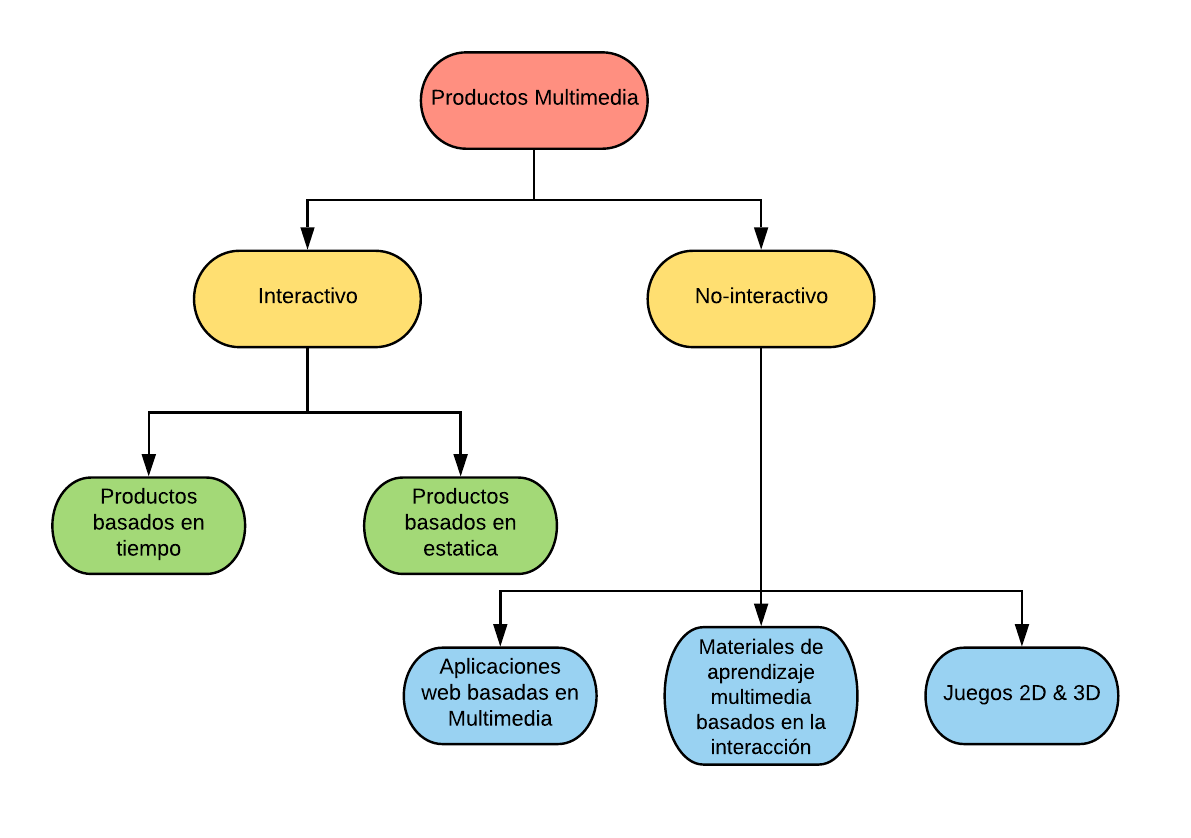
\includegraphics[width = 1\textwidth]{v2/images/image60.png}
 		\captionof{figure}{\label{fig:me2}Tipos de productos multimedia}
	\end{center} 
\end{figure}
Cada una de las categorías anteriores tiene un conjunto de características que pueden  clasificarse en tres dimensiones: vista externa, flujo de acciones y roles de los usuarios.\\
La vista externa se refiere a la forma en que el usuario interactúa con el producto. En este sentido, los usuarios interactúan con productos no interactivos de una manera.\\
Los usuarios suelen realizar eventos y la respuesta del producto a estos eventos mediante acciones.\\
%Un flujo de acciones se refiere al orden en que se muestran los marcos de los productos a los usuarios. En productos estáticos, no hay flujo de acciones, ya que los usuarios leen 
%ven un marco. Sin embargo, los flujos de acciones para productos basados ​​en el tiempo son una secuencia de cuadros. Por otro lado, el flujo de acciones 
%para los productos interactivos podría ser una secuencia, selectiva, iterativa e impulsada por eventos\cite{aleem2016game,cartwright1996pre}.\\
Los roles de los usuarios se refieren a lo que los usuarios pueden hacer para interactuar con productos multimedia. En los productos no interactivos, los usuarios son pasivos donde 
solo pueden leer / mirar productos. Sin embargo, los usuarios son usuarios activos con productos interactivos donde pueden realizar eventos. El cuadro \ref{tab:met1}  resume los tipos de productos 
multimedia y sus características.
\begin{table}[H]
  \resizebox{\textwidth}{!}{%
  \begin{tabular}{|
  >{\columncolor[HTML]{9B9B9B}}c |c|c|c|}
  \hline
  \cellcolor[HTML]{9B9B9B}                                                         & \multicolumn{3}{c|}{\cellcolor[HTML]{9B9B9B}\textbf{Características Multimedia}}                                                                                                                               \\ \cline{2-4} 
  \multirow{-2}{*}{\cellcolor[HTML]{9B9B9B}\textbf{Tipos de productos multimedia}} & \cellcolor[HTML]{9B9B9B}\textbf{Vista Externa} & \cellcolor[HTML]{9B9B9B}\textbf{Flujo de acciones}                                                   & \cellcolor[HTML]{9B9B9B}\textbf{Roles de los Usuarios} \\ \hline
  \textit{Productos estáticos}                                                     & Un cuadro                                      & Sin acciones                                                                                         & Pasivo (ver/leer)                                      \\ \hline
  \textit{Productos basados en tiempo}                                             & Múltiples cuadros                              & Secuencia                                                                                            & Pasivo(mirar)                                          \\ \hline
  \textit{Productos interactivos}                                                  & Impulsado por eventos                          & \begin{tabular}[c]{@{}c@{}}Secuencia, Selectiva, Interactiva e\\  Impulsada por eventos\end{tabular} & Activo(Realiza eventos)                                \\ \hline
  \end{tabular}%
  }
  \caption{Características de los productos multimedia.
  }
  \label{tab:met1}
  \end{table}

  \subsection{Características de la Metodología de ingeniería de software multimedia}
  \subsection{Requisitos y preproducción}
  El objetivo de esta fase es tener muy en claro cuales son los alcances y lo que será posible que el proyecto realice. Para ello se  realizaron las siguientes actividades:\\


\section{Selección de estrategia de diseño}
Al intentar comprender y desarrollar ideas relevantes para los temas, es necesario reiterar la comprensión de sus definiciones actuales y contexto histórico.\\
Con respecto a la realidad virtual, una de las cosas básicas a considerar es la forma en que nuestros sentidos sirven como la entrada que nuestro cerebro utiliza 
para construir una comprensión del mundo que nos rodea. La vista, el oído, el tacto, el olfato y el gusto son el conjunto de estímulo externo más ampliamente aceptado 
que percibe el cuerpo humano.\\
Estos sentidos y nuestras reacciones a ellos son el resultado de milenios de selección natural y hay varias consecuencias de esto incorporadas en nuestro instinto. 
Todo esto es un conocimiento relativamente común y parece que no es necesario reiterar aquí, pero lo importante es afirmar que nosotros, como humanos, tenemos ciertos 
resultados predecibles basados en ciertos conjuntos de entradas. Esencialmente, es instinto, naturaleza humana.\\
Un sitio web bien diseñado utilizará de manera similar el color, la distancia y la tipografía para comunicar claramente un propósito y, a menudo, persuadir algún tipo de acción.\\
Para que todo esto sea efectivo, se deben implementar y descubrir principios de diseño razonables. Existen varios principios para el diseño que pueden traducirse de otros medios. 
El diseño de impresión, el diseño web, la arquitectura, el diseño de interiores, el teatro, los gráficos en movimiento, etc., tienen elementos que pueden considerarse 
relevantes y adoptados. \cite{web18} \\
Al mismo tiempo, el medio de la realidad virtual como propiedades, como la capacidad de intersección del contenido, son únicas.\\
Es por esto que el diseño de un sistema de realidad virtual presenta retos los cuales son difíciles de sobrellevar ya que se tiene que crear una experiencia para el 
usuario en el sistema mismo lo cual conlleva a la selección de una estrategia de diseño centrada en la UX del usuario.

\section{Requisitos para el Desarrollo de Software para Proveer una Experiencia de Realidad Virtual Optima.}%Diseno de la experiencioa del usuario para RV
La realización una experiencia de realidad alternativa es la prueba definitiva para diseñar una experiencia de usuario impecable que pueda sumergir los sentidos y 
“engañar” a la mente para que abrace la falsa realidad. \\
Pero crear una experiencia de realidad virtual es mucho más complejo que la producción visual 2D y 3D normal asociada con películas y videojuegos, que nos presenta 
como desarrolladores y diseñadores un conjunto completamente nuevo de desafíos. Crear una experiencia de realidad virtual exitosa requiere que el pensamiento actual 
sobre UX evolucione para acomodar sus capacidades y requisitos ya que es una rama la cual, frecuentemente, no es estudiada a profundidad dentro de la carrera de 
Ingeniería en Sistemas Computacionales. 

\subsection{Los cuatro núcleos del diseño UX para RV}
Se plantean cuatro consideraciones centrales para el diseño de experiencias de realidad virtual:\\

\subsection{Interactivo y Reactivo}
La pantalla estereoscópica de visión amplia de los visores de realidad virtual, en este caso específico el Oculus Rift ®,  crea una imagen tridimensional que fomenta 
la profundidad y la perspectiva. El software RV debe seguir constantemente los movimientos de la cabeza y los ojos del usuario, permitiendo que las imágenes se muevan 
y cambien con cada nueva perspectiva, produciendo retroalimentación visual y creando una ilusión de sensación táctil.\\
La experiencia es altamente interactiva y reactiva porque el diseño responde a los movimientos de un usuario y, por lo tanto, siempre está cambiando.\\
Es por eso que una experiencia de realidad virtual se diseña a una vista de 360 grados. Cuando se está diseñando una experiencia, se debe de anticipar y dirigir cada 
movimiento del usuario, teniendo en cuenta dónde dirigir el ojo usando la vista, el sonido se presenta dentro del sistema que está proveyendo la experiencia de realidad virtual.

\subsection{Comodidad y Facilidad}
La cualidad más importante para crear cualquier diseño UX exitoso, especialmente en realidad virtual, es garantizar que el usuario se sienta cómodo durante toda la experiencia\cite{antonya2007design},
 lo que le permite tener un control completo de todos los movimientos y reducir la posibilidad de cinetosis.\\
Los cambios de brillo y los desajustes de velocidad son muy importantes. De hecho, la posibilidad de cinetosis fue un obstáculo importante para el desarrollo de la tecnología de 
Realidad Virtual.\\
Se debe implementar la capacidad de ver y usar controles, hacer clic en botones y otras características centradas en el diseño para evitar confundir o frustrar a los usuarios.\\
En otras palabras, dar al usuario la capacidad y la facilidad de controlar completamente su propia experiencia. Esa es la capacidad del sistema realidad virtual en el cual se 
intenta proveer la capacidad de experimentar completamente un mundo diferente y controlar cada uno de los movimientos del usuario dentro de ese mundo.

\subsection{Escala de texto e imagen}
La percepción actual de software realizado en realidad virtual es que este es "realista". Esto esencialmente está tratando de crear una experiencia que envuelve completamente al usuario.\\
Los detalles importan en el diseño de los sistemas, especialmente uno que sea lo suficientemente intuitivo para requerir la mínima curva de aprendizaje para el usuario.\\
Todas las imágenes deben ser claras y fácilmente legibles, evitando la fatiga visual y teniendo en cuenta la perspectiva. Agregar más y más detalles a un objeto a medida 
que el usuario se acerca a él ayudará a establecer una profundidad realista (y viceversa). El usuario notará mejor el texto grande, en negrita y colorido.

\subsection{Sonido}
La música y los efectos de sonido de alta calidad son una característica fundamental para fomentar la inmersión en la experiencia.\\
Mediante la implementación de 3D efectos de audio a RV audio posicional, el usuario sabrá la dirección en la que ciertos sonidos son originados en relación a donde están, 
o el audio podría ser hecho a sonar como es proveniente de todo tipo de direcciones, dando al usuario la ilusión de estar en medio de un entorno particular.\\
Dar a los usuarios un control de volumen también puede ser una buena idea para ayudar al usuario a encontrar un rango cómodo, aunque estos no son esenciales dentro del sistema.

\section{Retos de realidad virtual para anticipar}
A medida que los diseñadores y desarrolladores se sumergen más en la realidad virtual, este tipo de experiencia relativamente desconocida seguramente se utilizará de formas que 
aún no se han considerado y, por lo tanto, se tendrán desafíos y beneficios que aún no se han descubierto. Sin embargo, pruebas realizadas por usuarios\cite{wen19} han traído a la 
superficie desafíos de diseño actuales.\\
Si bien el objetivo de una experiencia de realidad virtual efectiva y placentera se logra utilizando los principios fundamentales de UX, crear realidad virtual es más fácil 
decirlo que hacerlo.\\
Al realizar el diseño se procura minimizar diligentemente las frustraciones y la confusión de los usuarios al agrupar los detalles y la funcionalidad del usuario en cada 
centímetro del diseño reactivo.

\subsection{Crear un Entorno que se Vea y se Sienta Real}
No ignorar ningún detalle y siempre dé a los usuarios un control completo. Un sistema de realidad virtual es altamente interactivo de 360 grados debe parecer tan realista que los 
usuarios olviden que es realidad virtual. \\
Ofrecer al usuario la capacidad de interactuar de todas las formas posibles, incluida la capacidad de tocar, levantar y lanzar todo tipo de objetos.

\subsection{Asegurar que los Usuarios no Sufran Cinetosis}
La cinetosis ocurre cuando las señales de movimiento físicas y visuales le dan al usuario información adversa. Las claves para evitar que los usuarios se enfermen por el movimiento 
mientras usan un sistema de realidad virtual son el seguimiento efectivo de la cabeza, que mantiene algunos objetos en posiciones fijas sin importar el movimiento del usuario.\\
Además, mantener una velocidad de fotogramas alta y nunca perder fotogramas. Otras formas de combatir la enfermedad de la simulación es minimizar el movimiento de la periferia 
en el diseño y no intentar acelerar al usuario (también conocido como: no simular cambios en la velocidad).

\subsection{Desarrollar controles y menús fáciles de usar}
Este es un desafío en el que los diseñadores todavía están trabajando y se ha diseñado de la mejor forma posible tomando en cuenta diferentes estrategias y modelos de diseño.\\
Dado que los menús de navegación y otros controles no se pueden colocar en las esquinas de la pantalla, ya que en un sistema de realidad virtual, no hay esquinas o puntos finales 
para su vista, deben permanecer fácilmente accesibles y fáciles de usar.\\
Algunos juegos de realidad virtual colocan los controles en las manos de realidad virtual del usuario y la navegación del menú se realiza con la cabeza.\\
Sea lo más creativo posible con la experimentación, pero si los controles y los menús son difíciles de operar o encontrar, lo más probable es que su diseño de RV reciba un gran 
reconocimiento de los usuarios. Un tutorial rápido antes de la experiencia puede ayudar a bordo del usuario para evitar la frustración.

\subsection{Mantener al usuario seguro}
Si bien los usuarios explorarán nuevos espacios, la realidad física es que el cuerpo del usuario todavía está atrapado dentro de una sala de la habitación donde se instale el sistema 
de realidad virtual.\\
Se tiene que asegurarse de que la experiencia de realidad virtual no representa serias amenazas de seguridad para los usuarios.\\
Hacer que funcione para los usuarios. Es importante tener en cuenta las diferentes alturas y tamaños de las personas. No colocar artículos críticos fuera del alcance de usuarios con 
una altura diferente. Además, se debe de tener en cuenta las diferentes preferencias y desventajas físicas al crear varios modos y permitir que los usuarios se sienten mientras visitan 
una realidad alternativa.

\section{Diseño y Desarrollo de Componentes Multimedia}
%se construyyeron modelos solidos basados en lo anterior  desarrollados en blender

\subsection{Modelos 3D de los Organos}
Los componentes multimedia a desarrollar en modelos 3D los cuales son miembros del sistema digestivo del ser humano, 
el sistema digestivo incluye a los órganos del tubo alimenticio y glándulas de secreción exocrina y endocrina.\\

\subsection{Glándulas Salivales}
 continuación se muestran las figuras del resultado final del desarrollo de las glándulas salivales del sistema digestivo 
 en el software de modelado en 3D llamado “Blender”, este fue realizado basado en el material anteriormente provisto.\\
\begin{figure}[H]
	\begin{center}
 		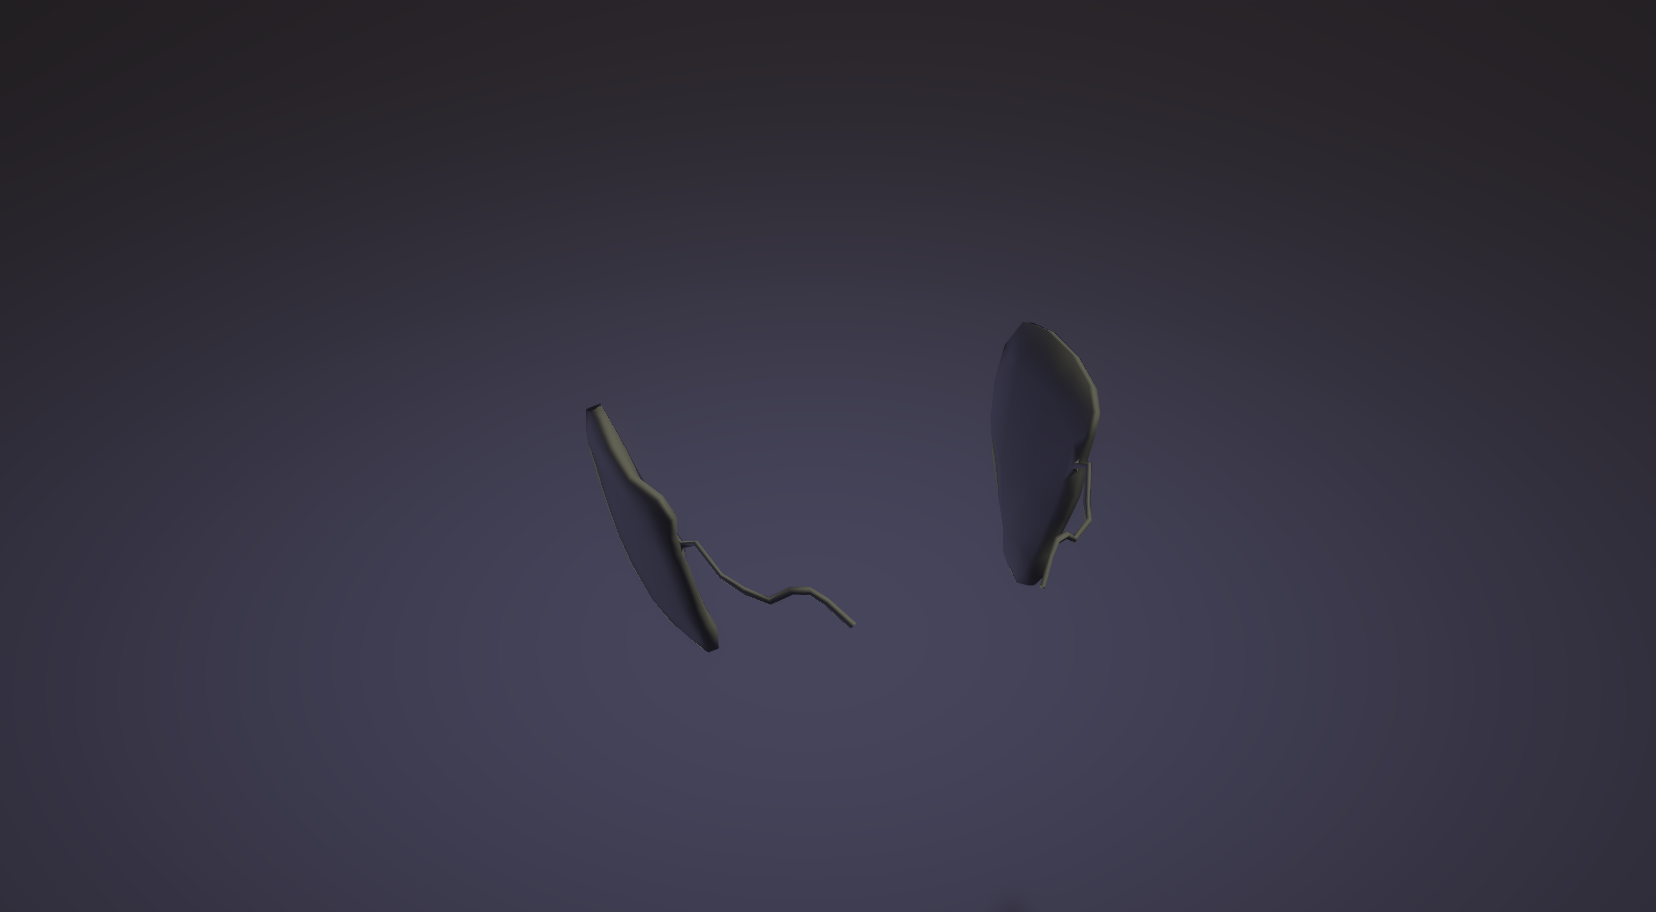
\includegraphics[width = .5\textwidth]{source/images/image41.png}
 		\captionof{figure}{\label{fig:im34}Modelo 3D de las glándulas salivales}
	\end{center} 
\end{figure}

\subsection{Cavidad oral y faringe}
A continuación se muestran las figuras del resultado final del desarrollo de la cavidad oral del sistema digestivo en el software de modelado en 3D llamado “Blender”, este fue realizado basado en el material anteriormente provisto.\\
\begin{figure}[H]
	\begin{center}
 		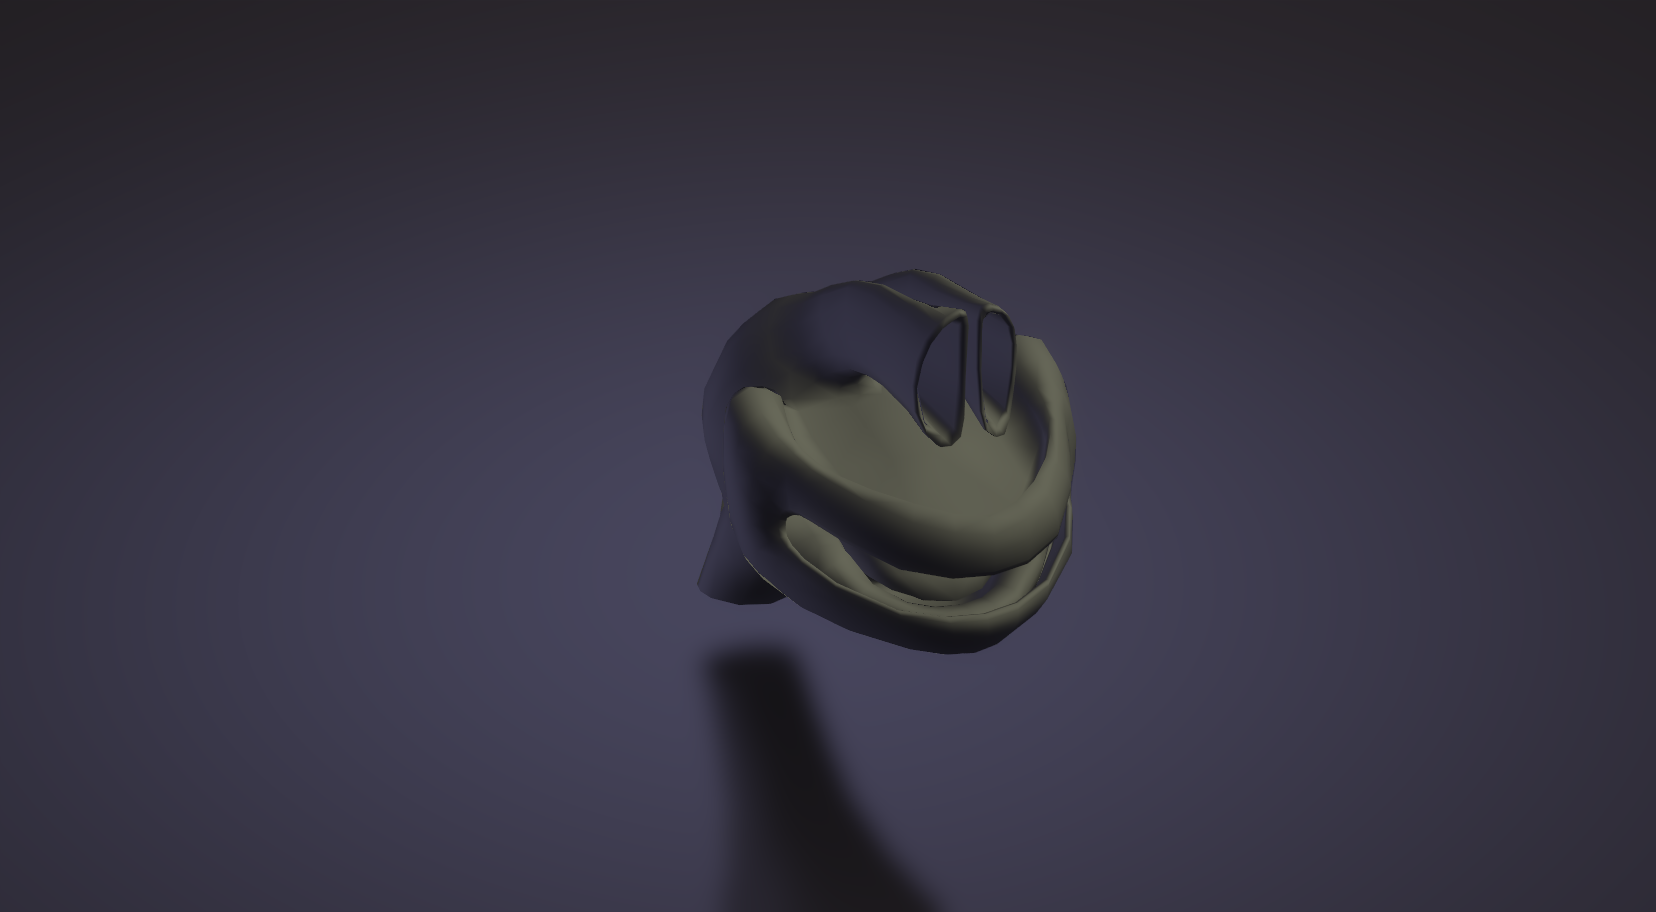
\includegraphics[width = .5\textwidth]{source/images/image14.png}
 		\captionof{figure}{\label{fig:im35}Modelo 3D de la cavidad oral}
	\end{center} 
\end{figure}

\subsection{Esófago}
A continuación se muestran las figuras del resultado final del desarrollo del esófago del sistema digestivo en el software de modelado en 3D llamado “Blender”, este fue realizado basado en el material anteriormente provisto.\\
\begin{figure}[H]
	\begin{center}
 		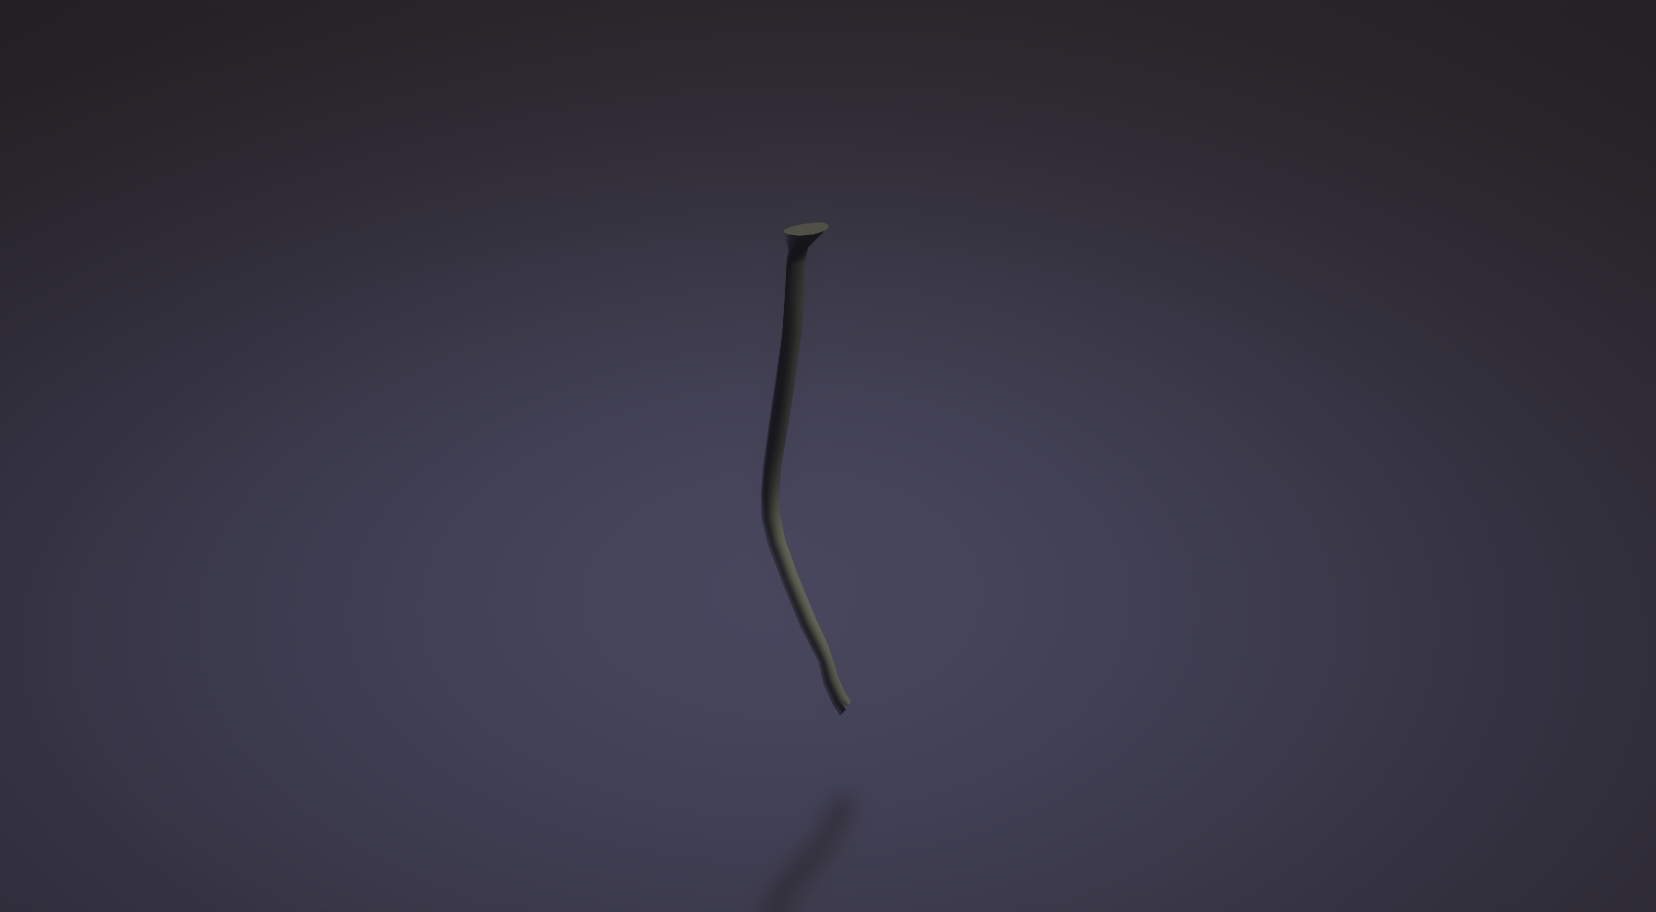
\includegraphics[width = .5\textwidth]{source/images/image25.png}
 		\captionof{figure}{\label{fig:im36}Modelo 3D del esófago}
	\end{center} 
\end{figure}

\subsection{Estómago}
A continuación se muestran las figuras del resultado final del desarrollo del estómago del sistema digestivo en el software de modelado en 3D llamado “Blender”, este fue realizado basado en el material anteriormente provisto.\\
\begin{figure}[H]
	\begin{center}
 		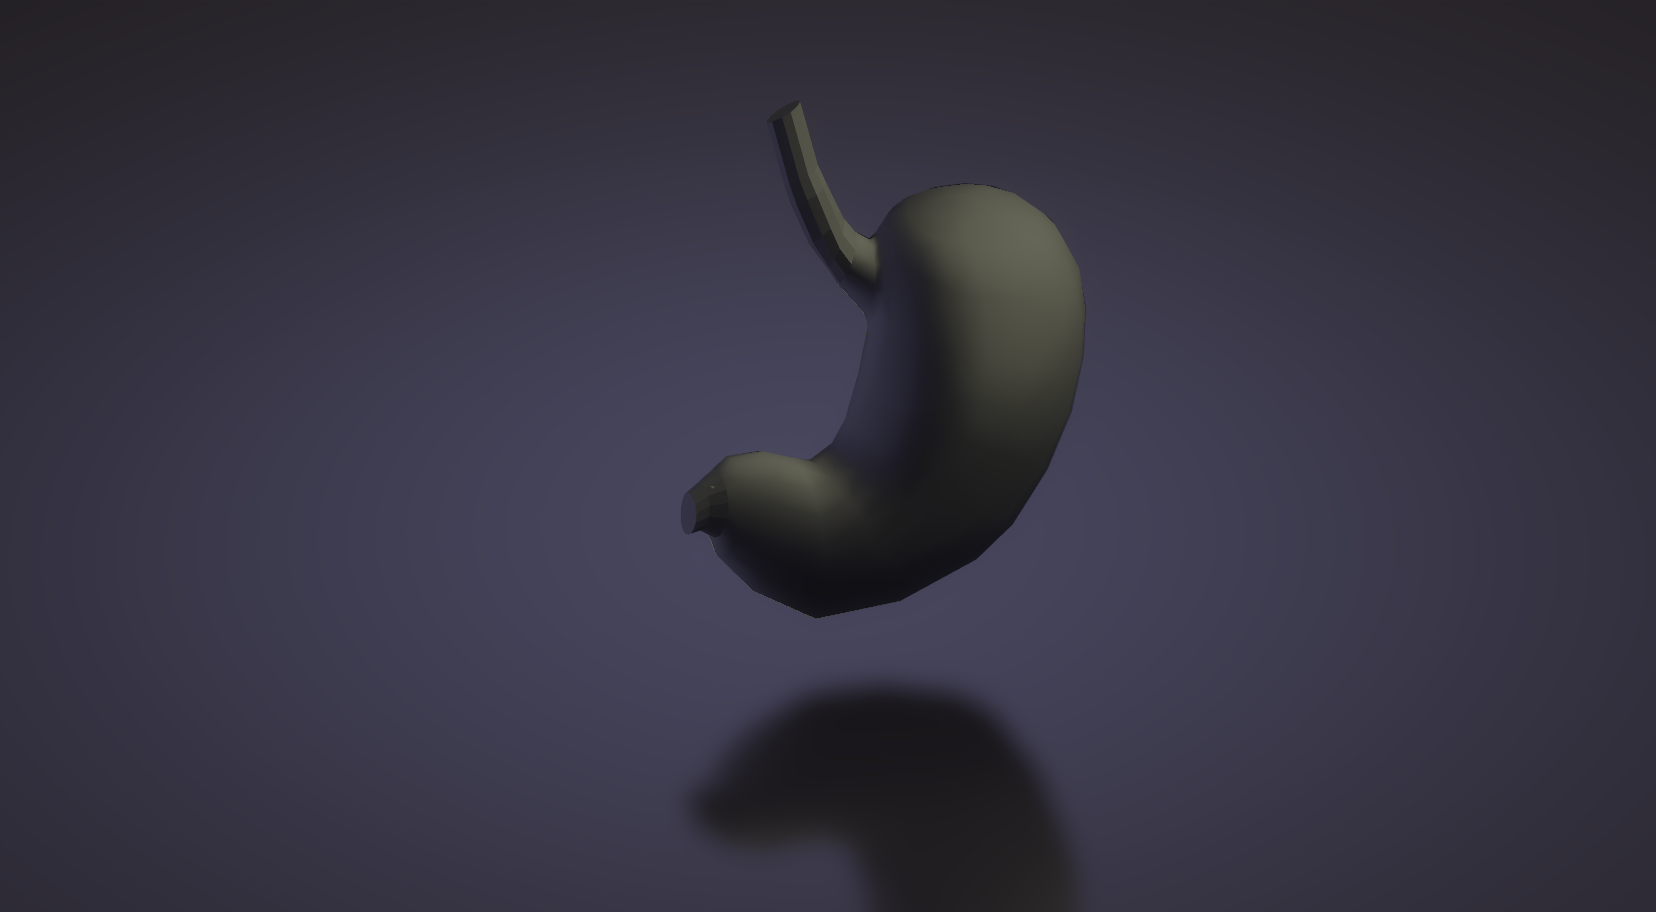
\includegraphics[width = .5\textwidth]{source/images/image42.png}
 		\captionof{figure}{\label{fig:im37} Modelo 3D del estómago }
	\end{center} 
\end{figure}

\subsection{Intestino delgado}
A continuación se muestran las figuras del resultado final del desarrollo del intestino delgado del sistema digestivo en el software de modelado en 3D llamado “Blender”, este fue realizado basado en el material anteriormente provisto.\\
\begin{figure}[H]
	\begin{center}
 		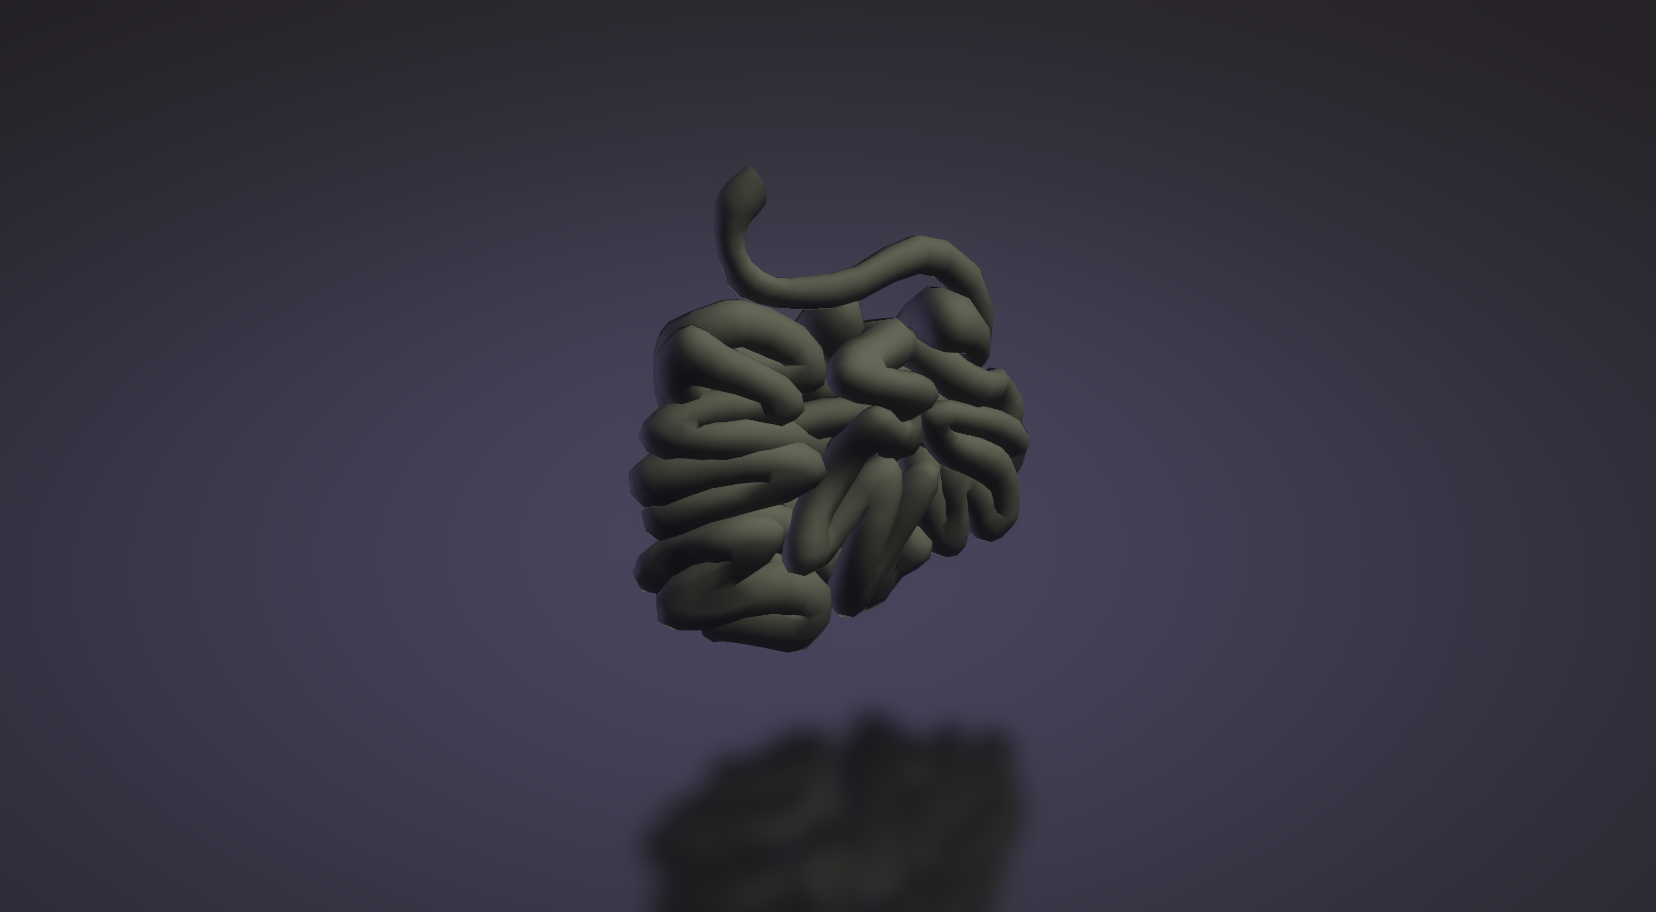
\includegraphics[width = .5\textwidth]{source/images/image69.png}
 		\captionof{figure}{\label{fig:im38}Modelo 3D del intestino delgado}
	\end{center} 
\end{figure}

\subsection{Hígado}
A continuación se muestran las figuras del resultado final del desarrollo del hígado del sistema digestivo en el software de modelado en 3D llamado “Blender”, este fue realizado basado en el material anteriormente provisto.\\
\begin{figure}[H]
	\begin{center}
 		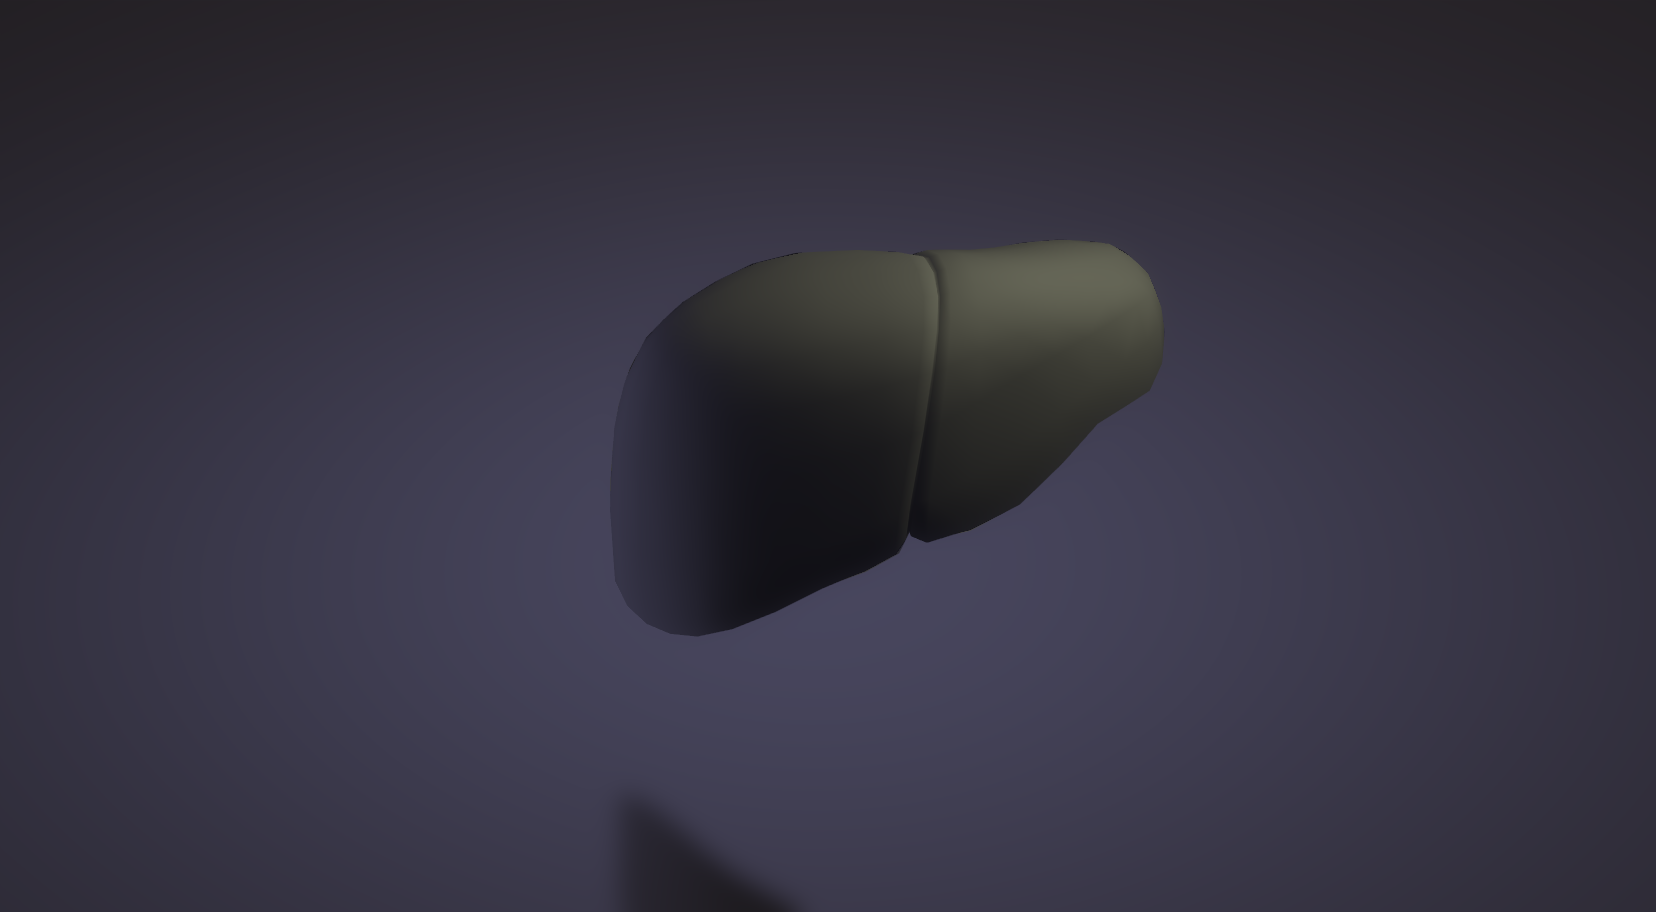
\includegraphics[width = .5\textwidth]{source/images/image17.png}
 		\captionof{figure}{\label{fig:im39}Modelo 3D del hígado}
	\end{center} 
\end{figure}

\subsection{Páncreas}
A continuación se muestran las figuras del resultado final del desarrollo del páncreas del sistema digestivo en el software de modelado en 3D llamado “Blender”, este fue realizado basado en el material anteriormente provisto.\\
\begin{figure}[H]
	\begin{center}
 		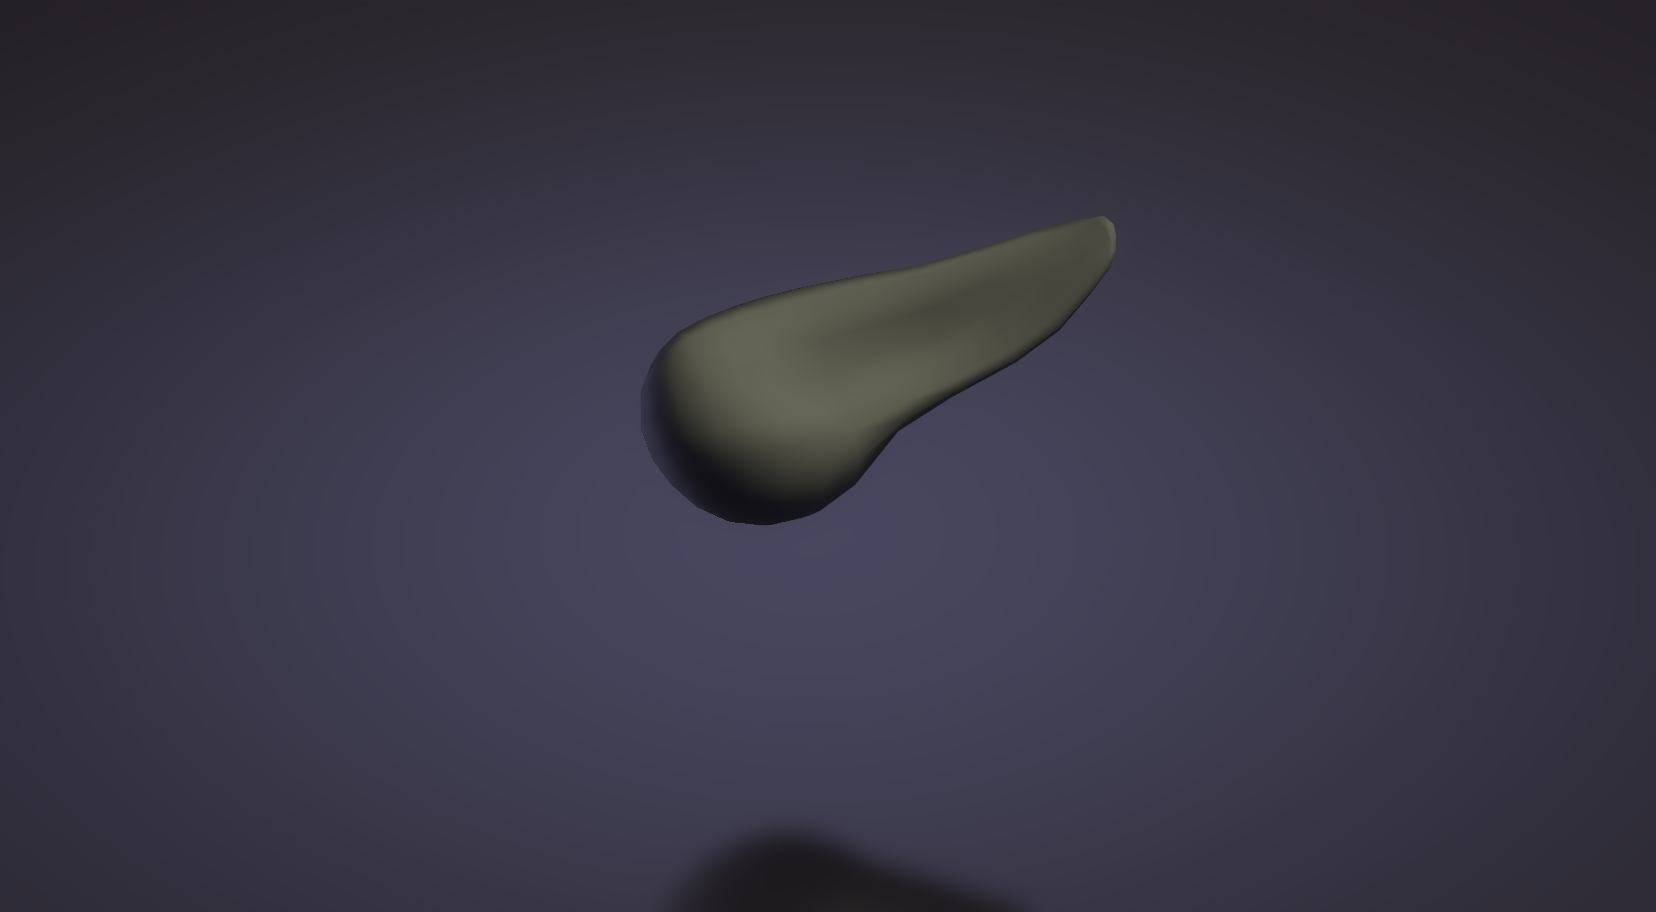
\includegraphics[width = .5\textwidth]{source/images/image19.png}
 		\captionof{figure}{\label{fig:im310}Modelo 3D del páncreas}
	\end{center} 
\end{figure}

\subsection{Vesícula Biliar}
A continuación se muestran las figuras del resultado final del desarrollo de la vesícula biliar del sistema digestivo en el software de modelado en 3D llamado “Blender”, este fue realizado basado en el material anteriormente provisto.\\
\begin{figure}[H]
	\begin{center}
 		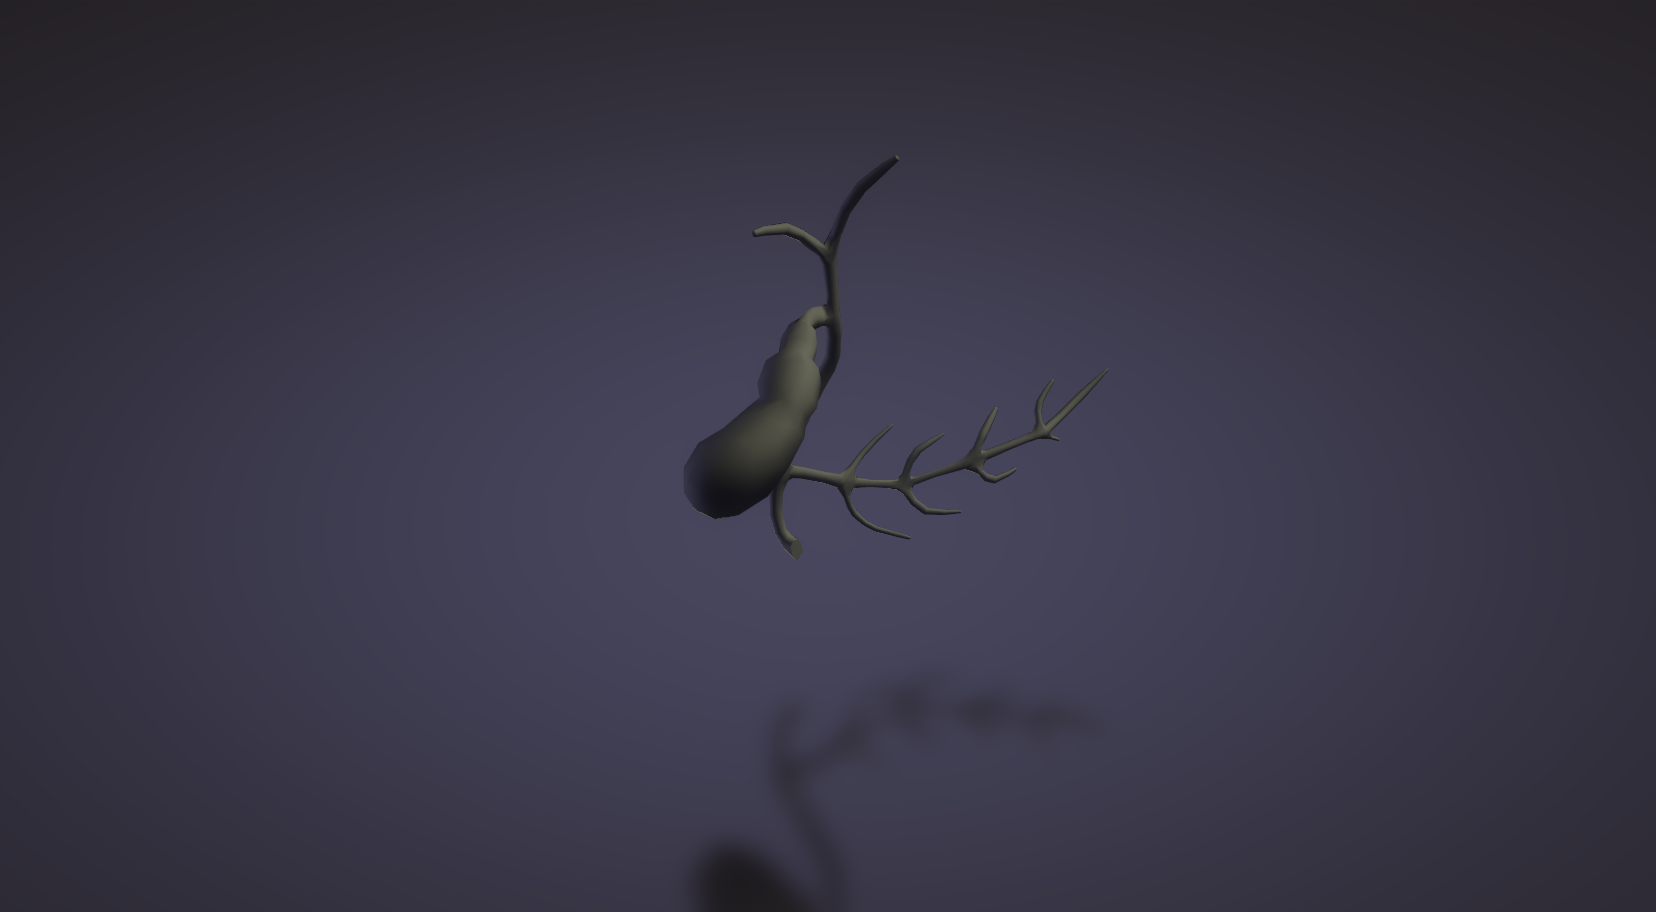
\includegraphics[width = .5\textwidth]{source/images/image26.png}
 		\captionof{figure}{\label{fig:im312}Modelo 3D de la vesícula biliar}
	\end{center} 
\end{figure}

\subsection{Intestino Grueso y Ano}
A continuación se muestran las figuras del resultado final del desarrollo del intestino grueso y ano del sistema digestivo en el software de modelado en 3D llamado “Blender”, este fue realizado basado en el material anteriormente provisto.\\
\begin{figure}[H]
	\begin{center}
 		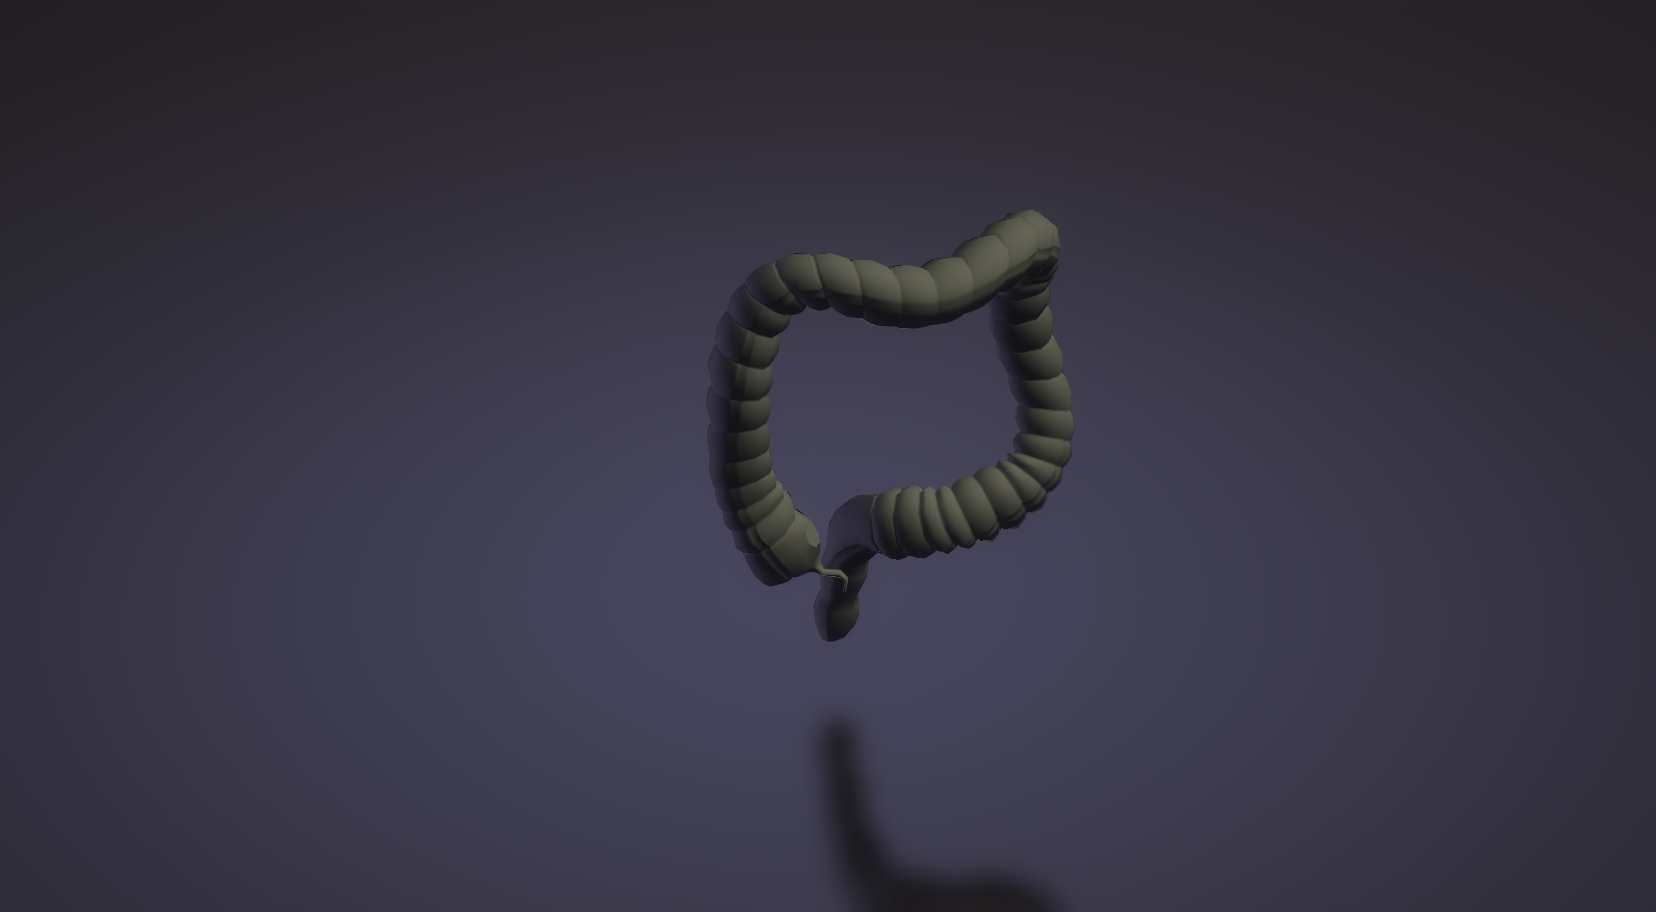
\includegraphics[width = .5\textwidth]{source/images/image20.png}
 		\captionof{figure}{\label{fig:im313}Modelo 3D del intestino grueso}
	\end{center} 
\end{figure}

\section{Modelo del sistema digestivo unificado}
A continuación se muestran las figuras del resultado final del desarrollo del sistema digestivo en el software de modelado en 3D llamado “Blender”, este fue realizado reuniendo todos los modelos de órganos y elementos individuales creados con anterioridad.\\
\begin{figure}[H]
	\begin{center}
 		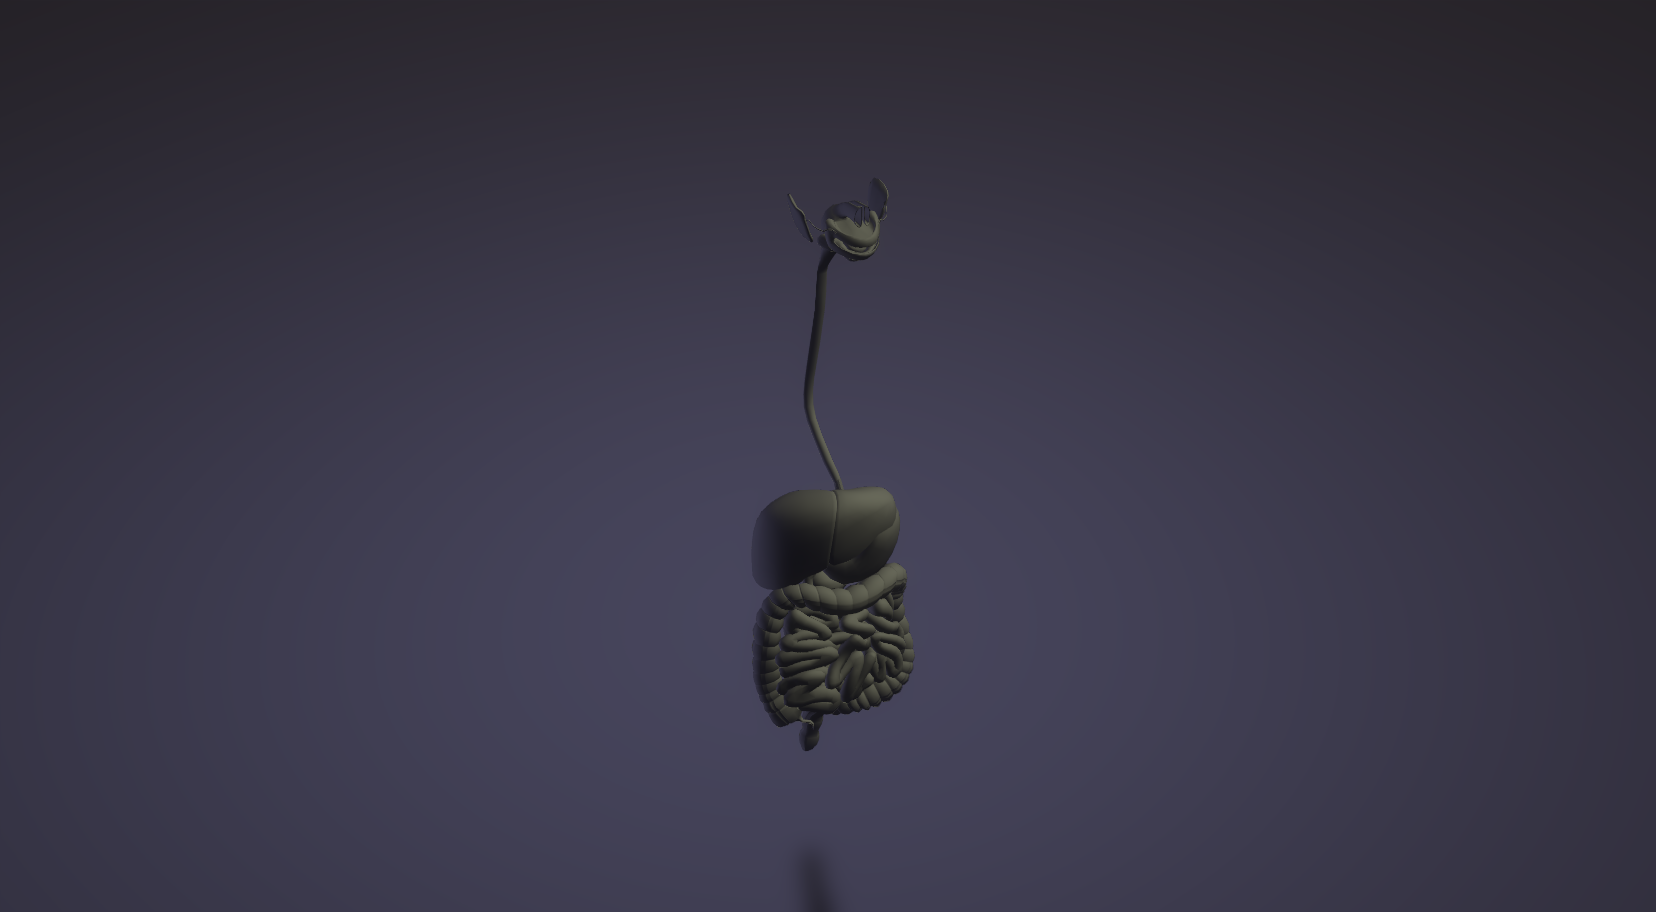
\includegraphics[width = 1\textwidth]{source/images/image24.png}
 		\captionof{figure}{\label{fig:im314}Modelo 3D del Sistema digestivo}
	\end{center} 
\end{figure}

\subsection{Generación de interacción con modelos 3D}
Para poder importar los modelos del sistema digestivo del cuerpo humano estos son agregados dentro de la misma carpeta del proyecto y seleccionar nuevo Asset.\\
Posteriormente estos se agregan a la escena principal del sistema, dependiendo de cuales son los que se deseen integrar.\\
Duplicando el objeto de escena del modelo 3D deseado y  se vuelve a pintar debajo del objeto Meshes en la jerarquía Interactable.Primary\_.Grab.Secondary\_.swap object y 
se ponga a cero los valores de transformación cuando sea necesario.\\
Se inhabilitó el objeto de escena original del modelo 3D deseado.\\
Si es necesario se ajusta la nueva transformación del modelo en 3D en los grados necesarios en el eje Y y se ajusta la transformación Interactable.Primary\_.Grab.Secondary 
swap object para ubicarse en el entorno 3D correctamente.\\
De esta manera se integran rápidamente los elementos multimedia diseñados anteriormente.\\
\begin{figure}[H]
	\begin{center}
 		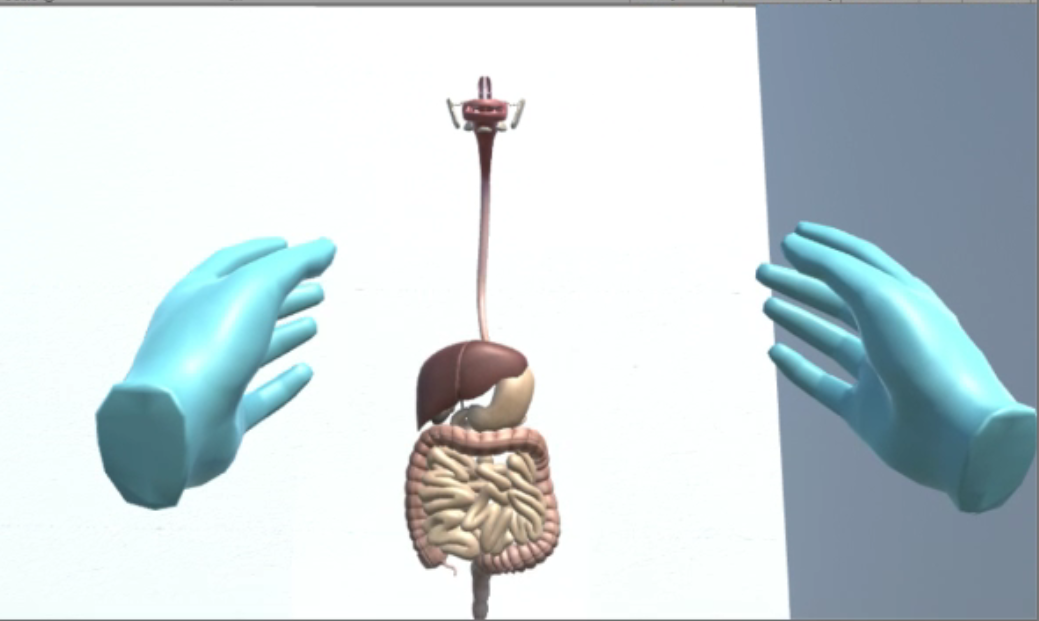
\includegraphics[width = .5\textwidth]{source/images/image37.png}
 		\captionof{figure}{\label{fig:im328}Integración de modelo del sistema digestivo 3D dentro del entorno 3D}
	\end{center} 
\end{figure}
\begin{figure}[H]
	\begin{center}
 		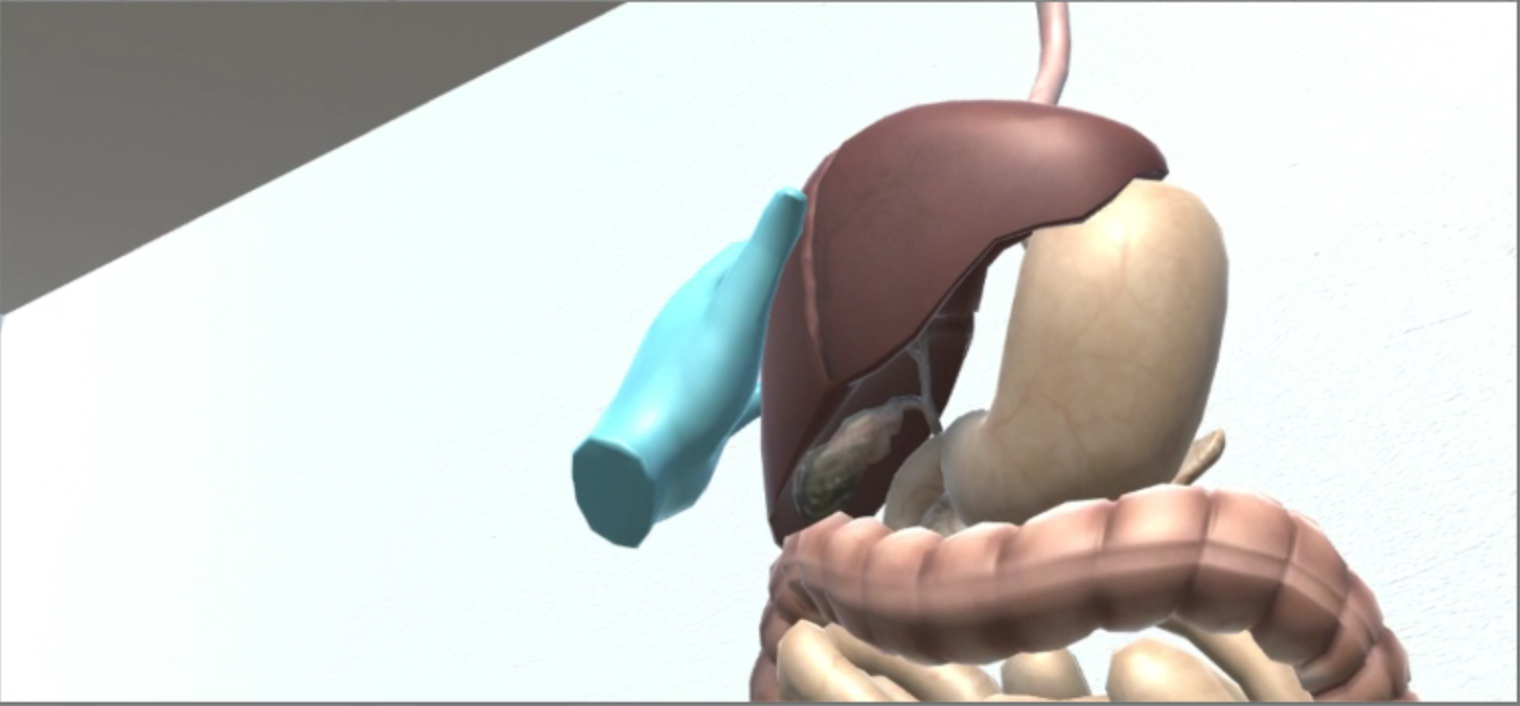
\includegraphics[width = .5\textwidth]{source/images/image67.png}
 		\captionof{figure}{\label{fig:im329}-  Interacción con modelo del hígado del sistema digestivo 3D dentro del entorno 3D}
	\end{center} 
\end{figure}

\section{Evaluación de modelos 3D por personal calificado}
Debido al tiempo de desarrollo, el cual tomó más de lo planteado, de los modelos antes expuestos en la sección anterior no fue posible concretar una cita 
para su evaluación con el personal calificado  de la Escuela Superior de Medicina en las fechas previamente planteadas.\\
Se esperaba poder tener una reunión en fechas posteriores pero la situación epidémica que se ha desarrollado en el país y 
limitaciones impuestas por las autoridades hicieron imposible la evaluación de los modelos desarrollados.\\
Esto no significa que no se haya hecho bajo rigor alguno, sólo se utilizaron materiales de medicina impresos, así como 
referencias en video de disecciones del sistema digestivo, esto para estar lo más familiarizado posible, como estudiante 
de ingeniería en sistemas computacionales, al momento de desarrollar dichos modelos.\\

\section{Diseño y Desarrollo de Componentes de Software}
Los componentes de software a diseñar y desarrollar el cual interactúa con el entorno en 3D y  modelos 3D.\\
Hubo puntos clave desarrollados los cuales tuvieron que ser desarrollada para llevar a cabo la mejor UX. Los desarrollos son incrementales, en cuanto a el grado de interacción 
que se logra.\\
Los componentes desarrollados para este software son:\\
\begin{itemize}
  \item Seguimiento de HMD y controles
  \item Locomoción y ergonomía
  \begin{itemize}
    \item Teleportación
    \item Puntos de teleportación
    \item Giros rápidos, entradas personalizadas, oclusión del usuario    
  \end{itemize}
  \item Presencia e interacción de las manos  
  \begin{itemize}
    \item Agregar manos
    \item Interactuando con entorno
    \item Interacciones manuales adicionales    
  \end{itemize}
\end{itemize}
Todos estos componentes forman la base para que la experiencia del software de realidad virtual se “sienta” lo más “natural” posible y estos mismos deben de estar refinados para que 
al integrarse con los componentes multimedia la interacción con estos se lleve de manera fluida.

\section{Creando el proyecto en Unity ®}
Se optó por el uso de Unity ® en su versión 2018.4 14f1 LTS  ya que esta misma será soportada por más tiempo y es ideal para un desarrollo en el cual se necesite solamente usar una versión estable del editor sin que haya cambios dentro de este que perjudique el desarrollo del sistema; así mismo es la versión que Oculus\cite{web15} recomienda dentro de sus requerimientos y recomendaciones de desarrollo.\\
\begin{figure}[H]
	\begin{center}
 		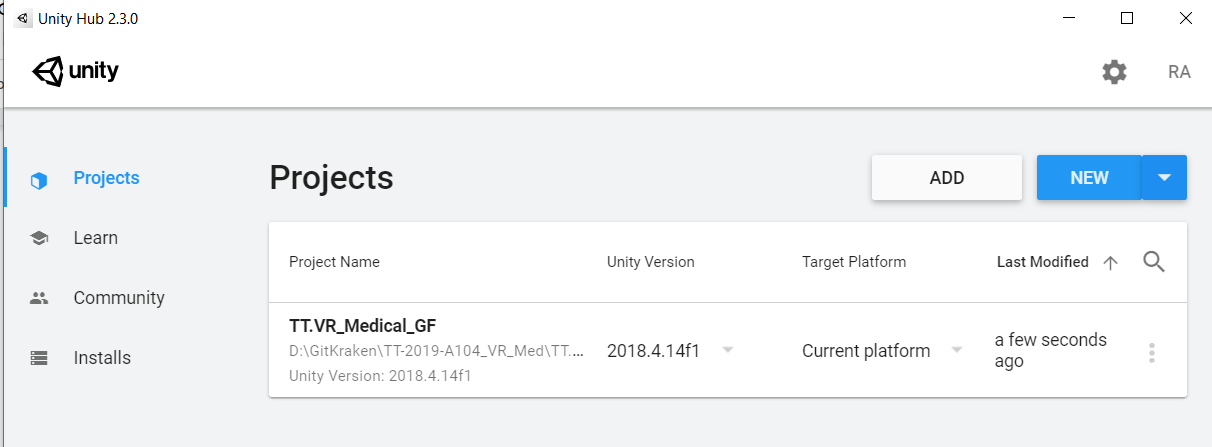
\includegraphics[width = 1\textwidth]{source/images/image51.png}
 		\captionof{figure}{\label{fig:im315}Unity Hub 2.3.0}
	\end{center} 
\end{figure}

\section{Seguimiento de HMD y controles}
En este apartado se realizó en rastreo del HMD y de los controles y que estos se vean reflejados como movimientos dentro del software y replicados en el mismo HMD el cual está siendo usado por el usuario y así puede percibir el movimiento. Esto es la base para que el software provea una experiencia en la cual el usuario pueda estar inmerso.\\

Utilizando el SDK que provee Oculus para su desarrollo con el motor Unity se realiza el elemento OVRCameraRig y TrackedAlias.\\

Se abrió el prefabricado OVRCameraRig , así como el objeto secundario TrackingSpace en la jerarquía. Se selecciona OVRCameraRig y luego se navega hasta el script LinkedAliasAssociationCollection en el inspector. Se adaptan los siguientes activos en las entradas apropiadas en el Script LinkedAliasAssociationCollection:\\
\begin{itemize}
    \item TrackingSpace a Play Area
    \item CenterEyeAnchor a el HMD
    \item CenterEyeAnchor a la cámara del HMD
    \item LeftHand Anchor al controlador izquierdo
    \item RightHandAnchor al controlador derecho
\end{itemize}
Realizando estos pasos se logra el rastreo de los controles y el HMD ejemplificando con la figura \ref{fig:im315.}.
\begin{figure}[H]
	\begin{center}
 		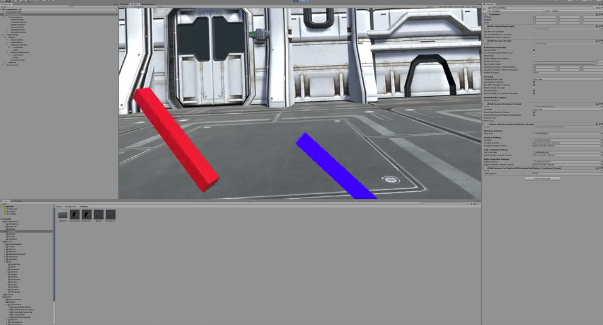
\includegraphics[width = .7\textwidth]{source/images/image44.png}
 		\captionof{figure}{\label{fig:im315.}Entorno de desarrollo Unity mostrando en rastreo del HMD y controles}
	\end{center} 
\end{figure}

\section{Locomoción y ergonomía}
El modo más simple de locomoción es el movimiento físico y este es el más confortable que se puede tener debido a que cuando uno decide moverse en la realidad el 
usuario también se moverá dentro del entorno virtual, pero este viene con limitaciones inherentes y retos que no son plenamente obvios al momento de la concepción y 
desarrollo, se exponen algunos a continuación .\\
\begin{itemize}
    \item Los usuarios poseen áreas de interacción de diferentes tamaños, no todos poseen un área grande lo cual les permite más libertad de movimiento, mientras más pequeño sea el espacio que requiera el usuario más usuarios podrán hacer uso del sistema. Se podría ajustar el contenido del sistema, pero esto implicaría mayor trabajo y tiempo, esto no se traduce en una experiencia de usuario mejor que si este se hubiera diseñado con un área de interacción pequeña en primer lugar.
    \item Se toma en cuenta que con el movimiento físico es probable que algunos usuarios no tengan la posibilidad de moverse físicamente dentro de su área, pueden estar limitados por una discapacidad, lo cual implicaría en que el movimiento sería una distracción para el usuario asumiendo que de algún modo este pudiera interactuar de alguna manera.
\end{itemize}
Otros dos tipos más de locomoción que se consideraron para el desarrollo del sistema uno de estos es el movimiento guionizado y movimiento de avatar, el primero se 
refiere a cuando la perspectiva se mueve a través de un camino predeterminado, este es usualmente utilizado cuando se realiza una experiencia que no requiera movimientos 
del usuario, fácilmente ejemplificado por un viaje en una montaña rusa en un software de realidad virtual este puede llegar a causar vección, generalmente este tipo de 
movimiento suele ser poco tolerable en largos periodos de tiempo.\\
Por otro lado el movimiento de avatar es el clásico movimiento que solemos encontrar en videojuegos o en experiencias pasadas de realidad virtual, al mover una palanca 
del mando el avatar comenzará su movimiento. Este fue un acercamiento más que válido pero con el progreso de la tecnología la manera de implementar el movimiento ha evolucionado.\\
La teleportación se refiere a una mecánica instantánea o casi instantánea en la cual el usuario aparece en un lugar seleccionado, típicamente funciona apuntando hacia al 
lugar deseado y presionando un botón, aunque hay múltiples variaciones de este acercamiento.\\
La teleportación ocurre en un instante lo cual reduce a un mínimo la posibilidad de generar una molestia comparación de los tipos de movimiento expuestos anteriormente.\\
Tomando en cuenta los tipos de movimiento pasado, sus deficiencias y beneficios se tomó la decisión de implementar la teleportación como método de movimiento en el entorno 
virtual del sistema.\\

\subsection{Teleportación}
En este apartado se desarrollaron los movimientos que el usuario pudiera tener dentro del entorno en 3D, estos dan la posibilidad de “movimiento” dentro del mismo así 
como las limitaciones que se implementan para que el mismo usuario no pueda acceder a partes que no queramos o estén disponibles para este.\\
El desarrollo se realizó de la manera siguiente:\\ 
Se cambió el nombre del Prefab a una convención de nombres, en este caso Teleport.Curved. respectivamente, y se realizó una copia para la mano derecha para tener 
un objeto distinto para la mano derecha.\\
Se configuró el script de fachada de puntero adjunto a cada objeto arrastrando el Alias de controlador correspondiente de la Jerarquía al campo FollowSource.\\
Se crearon dos nuevos GameObjects vacíos para el manejo de las entradas del control y adjunto el script OVRInputTouchAction a cada uno de ellos.\\
Se estableció el valor de la propiedad táctil de ambos scripts OVRInputTouchAction en Thumbstick primario. Estableciendo el valor de la propiedad del controlador en L Touch
 y R Touch respectivamente.\\

\begin{verbatim}
    using System.Collections;
using System.Collections.Generic;
using UnityEngine;
using Zinnia.Action;
 
public class OVRInputTouchAction : BooleanAction
{
    public OVRInput.Controller controller = OVRInput.Controller.Active;
    public OVRInput.Touch touch;
 
    void Update() {
        Receive(OVRInput.Get(touch, controller));
    }
}
\end{verbatim}
Para cada objeto de ObjectPointer.Curved, se le asigna el objeto TeleportCurved correspondiente de la Jerarquía con un script OVRInputTouch al campo Acción de activación en el componente Fachada de puntero.\\

De esta manera al tocar cualquier thumbstick este invocará una curva la cual nos mostrará dónde será la teleportación una vez esta sea implementada.\\
\begin{figure}[H]
	\begin{center}
 		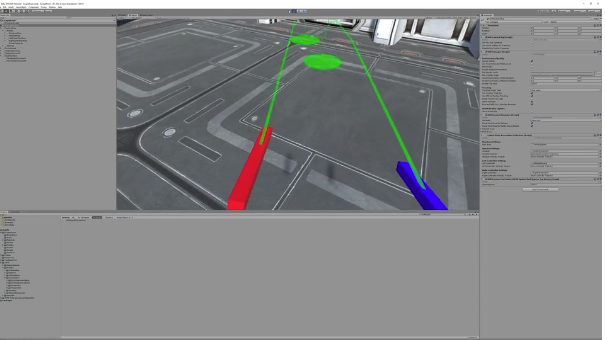
\includegraphics[width = .5\textwidth]{source/images/image73.png}
 		\captionof{figure}{\label{fig:im316}Curva que muestra la ubicación de la teleportación al tocar los thumbstick de los controles.}
	\end{center} 
\end{figure}

Para la adición de la acción de teleportación, la cual es la que permitirá el movimiento del usuario dentro del entorno de realidad virtual. Se tuvo la opción de 
implementar dos tipos de acciones de teleportación, Teleport.Instant y Teleport.Dash, se eligió la primera ya que supone una menor probabilidad de causar vección en el usuario 
 a que no se percibe movimiento alguno en la acción de teleportación.\\
Se implementó VRTK/Locomotion/Teleporter y arrastrando el Teleporter.Prefab instantánea a la escena.\\
%En el script de TeleporterFacade se adjunto al objeto Teleporter.Instant, asignado al objeto de  la escena PlayAreaAlias ​​al campo Target y el objeto de escena HeadsetAlias ​​al campo Offset.\\
Se estableció el campo de validez de la cámara del script de TeleporterFacade en el objeto de escena SceneCameras.\\
Se crearon dos nuevos GameObjects vacíos  para adjuntar las entradas de los botones y se adjunto el script OVRInputButtonAction a cada uno de ellos.\\
Se estableció el valor de la propiedad táctil de ambos scripts OVRInputButtonAction en Thumbstick primario. Se estableció el valor de la propiedad del controlador en 
L.Touch y R.Touch respectivamente.\\

\begin{verbatim}
    using System.Collections.Generic;
using UnityEngine;
using Zinnia.Action;
 
public class OVRInputButtonAction : BooleanAction {
    public OVRInput.Controller controller = OVRInput.Controller.Active;
    public OVRInput.Button button;
 
    void Update() {
        Receive(OVRInput.Get(button, controller));
    }
}
\end{verbatim}

Para cada objeto prefabricado Curva de puntero de objeto, se asignó los GameObjects correspondientes con el script OVRInputButtonAction al campo Acción de selección en el 
componente Fachada de puntero.\\
Para cada puntero de ObjectPointer.Curved, se agregó un nuevo objeto EventData en la lista Datos de acción seleccionados.\\
Se asignó el objeto Teleporter.Instant al campo de objeto ubicando y seleccionando TeleporterFacade y luego Teleport.\\
Implementando los procesos pasados se logra que el usuario pueda teleportarse dentro del  entorno virtual.\\
De esta manera al tocar cualquier thumbstick este invocará una curva la cual nos mostrará dónde será la teleportación una vez esta sea implementada.\\
\begin{figure}[H]
	\begin{center}
 		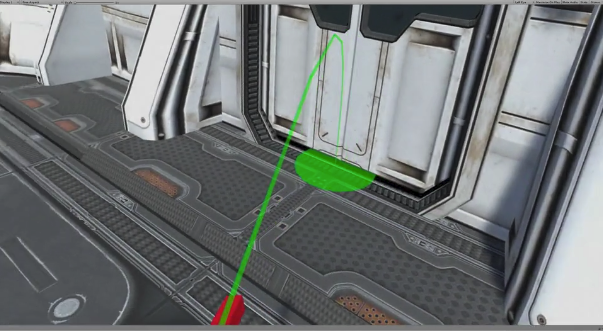
\includegraphics[width = .5\textwidth]{source/images/image35.png}
 		\captionof{figure}{\label{fig:im317}Curva que muestra la ubicación de la teleportación al tocar los thumbstick del control izquierdo.}
	\end{center} 
\end{figure}
\begin{figure}[H]
	\begin{center}
 		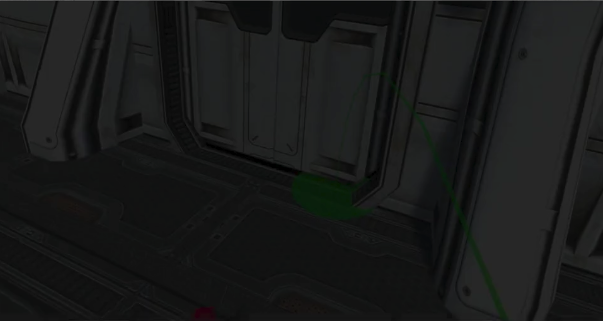
\includegraphics[width = .5\textwidth]{source/images/image61.png}
 		\captionof{figure}{\label{fig:im318}Curva que muestra la ubicación de la teleportación al tocar los thumbstick de los controles.}
	\end{center} 
\end{figure}

En la figura \ref{fig:im318} se puede notar un oscurecimiento, el cual es representativo del desvanecimiento que se implementó para reducir la vección del usuario y evitar 
cinetosis en los usuarios que pudieran llegar a ser propensos a ella.\\
Se procedió a integrar un indicador de flecha el cual servirá para indicar a de cara a que posición se estará cuando se realice la teleportación, así ampliando las posibilidades 
de interacción del usuario y facilitando las mismas.\\
Se importó un modelo de flecha en la vista Proyecto y fue arrastrado a la escena debajo del objeto de escena ValidContainer ubicado dentro de la jerarquía de objetos de escena 
de Destino para cada prefab ObjectPointerCurved.\\
Se ajustó la transformación del nuevo objeto de flecha para que sea visible dentro de la escena y asigne material PointerDefaultValid al renderizador de malla.\\
Se crearon dos nuevos GameObjects para cada control y obtener la dirección del stick del control vacíos y integró el script OVRInputAxis2DAction a cada uno de ellos.\\
Se estableció el valor de la propiedad táctil de ambos scripts OVRInputAxis2DAction en el control primario así como el valor de la propiedad del controlador en L Touch 
y R Touch respectivamente.\\
Se implementa el prefabricado AxisRotator a la escena.\\
Se cambia el nombre del Prefab a una convención de nombres AxisRotator.L  y se realiza una copia para la mano derecha ya se que implemento de la misma manera con el nombre AxisRotator.R\\
Se crearon dos nuevos GameObjects vacíos debajo de cada uno de los objetos OVRInputAxis2DAction creados anteriormente y se agrego el script Vector2ToFloat a los cuatro.\\

\begin{verbatim}
    using System.Collections;
using System.Collections.Generic;
using UnityEngine;
using Zinnia.Action;
 
public class OVRInputAxis2DAction : Vector2Action
{
    public OVRInput.Controller controller = OVRInput.Controller.Active;
    public OVRInput.Axis2D axis;
 
    void Update() {
        Receive(OVRInput.Get(axis, controller));
    }
}
\end{verbatim}

Se estableció el valor del eje del script Vector2ToFloat en el eje correcto, en este caso, una X y una Y para cada objeto OVRInputAxis2DAction.\\
En cada secuencia de comandos OVRInputAxis2DAction, se agregaron dos nuevos objetos Vector2 a la lista de valores cambiados de Vector2.\\
Se asignaron los objetos Vector2ToFloat a cada campo. Usando el menú desplegable, seleccione Vector2ToFloat y luego DoTransform.\\
Use el botón "Agregar componente" en el Inspector para agregar el componente de script FloatAction a cada objeto Vector2ToFloat.\\
En cada scriptVector2ToFloat, agregue un nuevo objeto de acción individual a la lista de acciones individuales transformadas y asigne el objeto primario.\\
Usando el menú desplegable, seleccione FloatAction y luego Recibir.\\
Se configuró cada objeto AxisRotator asignando un objeto FloatAction en los campos Eje lateral lateral y Eje longitudinal correspondientes en el script AxisRotatorFacade 
para los ejes X e Y de cada mano, respectivamente.\\
%En cada script AxisRotatorFacade, se asignó el objeto de escena ValidContainer correspondiente que se encuentra en la Jerarquía de cada prefabricado ObjectPointerCurved al campo Destino. Se asignó el objeto HeadsetAlias ​​al campo Offset direccional en cada uno de los scripts de AxisRotatorFacade.
En la secuencia de comandos de TeleporterFacade, establezca el valor de Uso de desplazamiento en Offset siempre con rotación de destino.\\
Implementando esto se logra que un puntero aparezca en una flecha en la dirección indicada para que el usuario pueda elegir su dirección de orientación al 
elegir la ubicación de teleportación como se muestra en la figura \ref{fig:im319}.\\

\begin{figure}[H]
	\begin{center}
 		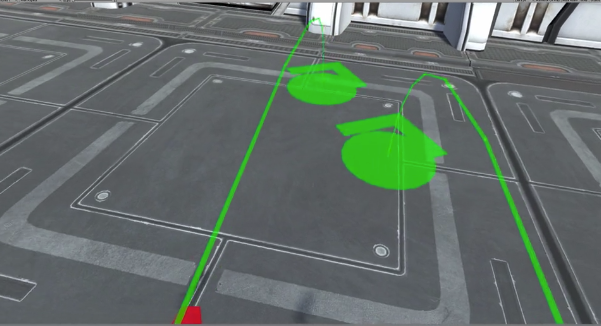
\includegraphics[width = .5\textwidth]{source/images/image62.png}
 		\captionof{figure}{\label{fig:im319}Curva que muestra la ubicación de la teleportación y posición del stick al interactuar con los thumbstick de los controles}
	\end{center} 
\end{figure}
\begin{figure}[H]
	\begin{center}
 		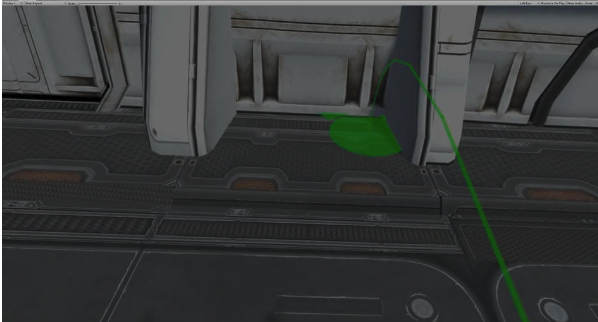
\includegraphics[width = .5\textwidth]{source/images/image4.png}
 		\captionof{figure}{\label{fig:im320}Curva que muestra la ubicación de la teleportación y posición del stick al interactuar con los thumbstick de los controles}
	\end{center} 
\end{figure}

\subsection{Puntos de teleportación}
Los puntos de teleportación son los cuales resaltan una locación dentro del entorno virtual la cual se quiere o requiere que el usuario vaya con facilidad hacia ellas.\\
Se agregó una nueva capa llamada "Teleportable" y se estableció el objeto FloorCollider en la nueva capa.\\
Se creó un nuevo GameObject vacío y se agregaron componente en el Inspector para adjuntar el script AnyLayerRule.\\
Se estableció el campo LayerMask en el script AnyLayerRule en la capa Teleportable.\\
\begin{verbatim}
    namespace VRTK.Prefabs.Locomotion.DestinationLocations
{
    using UnityEngine;
    using UnityEngine.Events;
    using Malimbe.MemberChangeMethod;
    using Malimbe.MemberClearanceMethod;
    using Malimbe.XmlDocumentationAttribute;
    using Malimbe.PropertySerializationAttribute;
    using Zinnia.Rule;
    using Zinnia.Data.Attribute;
 
    /// <summary>
    /// The public interface into the DestinationLocation Prefab.
    /// </summary>
    public class DestinationLocationFacade : MonoBehaviour
    {
        #region Location Settings
        /// <summary>
        /// Determines if the location is in the locked and unusable state.
        /// </summary>
        [Serialized]
        [field: Header("Location Settings"), DocumentedByXml]
        public bool IsLocked { get; set; }
        /// <summary>
        /// Whether to apply the rotation of the custom destination location to the selected action output.
        /// </summary>
        [Serialized]
        [field: DocumentedByXml]
        public bool ApplyDestinationRotation { get; set; } = true;
        /// <summary>
        /// Allows to optionally determine which <see cref="SurfaceData"/> sources can affect the location.
        /// </summary>
        [Serialized, Cleared]
        [field: DocumentedByXml]
        public RuleContainer SourceValidity { get; set; }
        #endregion
 
        #region Location Events
        /// <summary>
        /// Emitted when the Destination Location is entered for the first time.
        /// </summary>
        [Header("Location Events"), DocumentedByXml]
        public UnityEvent HoverActivated = new UnityEvent();
        /// <summary>
        /// Emitted when the Destination Location is entered.
        /// </summary>
        [DocumentedByXml]
        public DestinationLocation.SurfaceDataUnityEvent Entered = new DestinationLocation.SurfaceDataUnityEvent();
        /// <summary>
        /// Emitted when the Destination Location is exited.
        /// </summary>
        [DocumentedByXml]
        public DestinationLocation.SurfaceDataUnityEvent Exited = new DestinationLocation.SurfaceDataUnityEvent();
        /// <summary>
        /// Emitted when the Destination Location is exited for the last time.
        /// </summary>
        [DocumentedByXml]
        public UnityEvent HoverDeactivated = new UnityEvent();
        /// <summary>
        /// Emitted when the Destination Location is activated.
        /// </summary>
        [DocumentedByXml]
        public DestinationLocation.TransformDataUnityEvent Activated = new DestinationLocation.TransformDataUnityEvent();
        /// <summary>
        /// Emitted when the Destination Location is deactivated.
        /// </summary>
        [DocumentedByXml]
        public UnityEvent Deactivated = new UnityEvent();
        #endregion
 
        #region Reference Settings
        /// <summary>
        /// The linked Internal Setup.
        /// </summary>
        [Serialized, Cleared]
        [field: Header("Reference Settings"), DocumentedByXml, Restricted]
        public DestinationLocationConfigurator Configuration { get; protected set; }
        #endregion
 
        /// <summary>
        /// Called after <see cref="IsLocked"/> has been changed.
        /// </summary>
        [CalledAfterChangeOf(nameof(IsLocked))]
        protected virtual void OnAfterIsLockedChange()
        {
            Configuration.SetLockedState(IsLocked);
        }
 
        /// <summary>
        /// Called after <see cref="ApplyDestinationRotation"/> has been changed.
        /// </summary>
        [CalledAfterChangeOf(nameof(ApplyDestinationRotation))]
        protected virtual void OnAfterApplyDestinationRotationChange()
        {
            Configuration.LocationController.ApplyDestinationRotation = ApplyDestinationRotation;
        }
 
        /// <summary>
        /// Called after <see cref="SourceValidity"/> has been changed.
        /// </summary>
        [CalledAfterChangeOf(nameof(SourceValidity))]
        protected virtual void OnAfterSourceValidityChange()
        {
            Configuration.LocationController.SourceValidity = SourceValidity;
        }
    }
}
\end{verbatim}
Se estableció el campo TargetValidity en el script TeleporterFacade en AnyLayerRule script gameobject.\\

Para cada ObjectPointerCurved, se asigno AnyLayerRule al campo TargetValidity del script PointerFacade.\\
\begin{figure}[H]
	\begin{center}
 		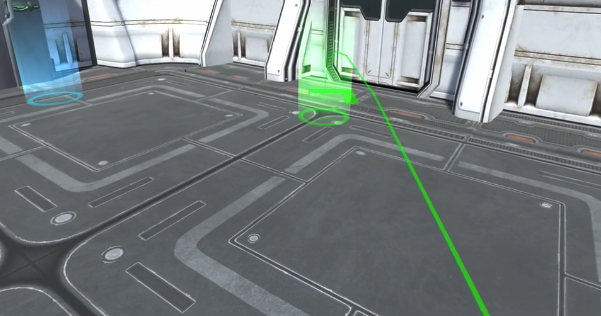
\includegraphics[width = .5\textwidth]{source/images/image45.png}
 		\captionof{figure}{\label{fig:im321}Desvanecimiento al realizar la teleportación y posición del stick al interactuar con los thumbstick del control}
	\end{center} 
\end{figure}

\subsection{Giros rápidos, entradas personalizadas, oclusión del usuario}
En esta sección se implementan giros de la cámara para facilitar al usuario la interacción en el entorno virtual así como la personalización y mejoras de interacción 
con los controles las cuales pretenden hacer más intuitivo el movimiento del usuario en el sistema de realidad virtual, además se implementan oclusiones en determinados 
lugares para evitar que el mismo usuario pueda ver a través de modelos 3D no deseados mermando así la experiencia de usuario.\\
Se creó un nuevo GameObject vacío para obtener  cuando el stick es tocado y adjunto el script de TeleporterActivation y configurando el campo Controlador en R Touch.\\
Se creó otro nuevo GameObject vacío y adjunto la secuencia de comandos TeleporterSelection y configuro el campo Controlador en R Touch.\\ 
Se crearon dos nuevos GameObjects vacíos para ser agregados al InputHandler bajo el script TeleporterSelection GameObject y  adjuntó el script FloatAction a cada uno.\\
Se agregó el componente en el Inspector para agregar los objetos del juego de script FloatAction a los campos Extraer X e Extraer Y del script TeleporterSelection.\\
Se asignaron los campos Eje lateral y Eje longitudinal en la secuencia de comandos AxisRotatorFacade a las dos nuevas secuencias de comandos de FloatAction GameObjects.\\
Fueron deshabilitados los objetos de juego de script OVRInputTouch, OVRInputButtonAction y OVRIInputAxis2DAction para la mano derecha.\\
Fueron reasignados los campos Acción de activación y Acción de selección en la secuencia de comandos de PointerFacade de la derecha a la secuencia de comandos 
TeleporterActivation y TeleporterSelection GameObjects, respectivamente.\\
Se inhabilitó el prefabricado ObjectPointerCurved de la izquierda en la escena y el script OVRInputTouch, OVRInputButtonAction GameObjects para la mano izquierda.\\
\begin{figure}[H]
	\begin{center}
 		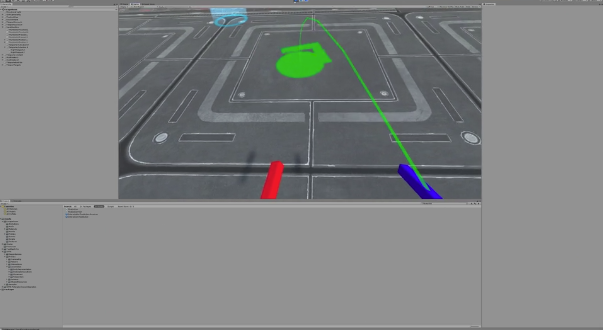
\includegraphics[width = .5\textwidth]{source/images/image57.png}
 		\captionof{figure}{\label{fig:im322} Curva de teleportación habilitada solamente para el control derecho}
	\end{center} 
\end{figure}

En el script AxesToVector3Facade adjunto al PrefabObject, estableciendo el Tipo de uso del eje Direccional.\\
Se  estableció el campo Eje lateral en el valor del eje X FloatAction script GameObject ubicado debajo de la mano izquierda OVRInputAxis2DAction script GameObject.\\
Se estableció el valor del campo Multiplicador de velocidad lateral en 45 y el valor del campo Multiplicador de velocidad longitudinal en 0.\\
Agregando una secuencia de comandos Vector3Cache a la secuencia de comandos AxesToVector3Facade GameObject.\\
Se agregó una nueva acción Vector3 a la lista de acciones Vector3 procesadas en el script AxesToVector3Facade y fueron agregadas al GameObject padre. 
Estableciendo las funciones en Vector3Cache/CachedData.\\
Fue agregado un script CameraColorOverlay al script GameObject de AxesToVector3Facade.\\
Se agregó un nuevo Vector3 a la lista de Vector3 modificado en el script Vector3Cache y  se agrego el objeto del juego principal. Estableciendo las funciones en CameraColorOverlay/link.\\
En el script CameraColorOverlay, se asignó el objeto de escena SceneCameras al campo Validez de la cámara.\\
Se implementó el material de TeleportFade en el proyecto y asignando al campo Material de superposición en el script CameraColorOverlay y cambie el valor del campo Eliminar duración a 0.5.\\
Se creó un nuevo GameObject vacío y se agrego el componente para agregar el script Vector3ToVector2 y un script Vector2ToVector3.\\
Fue agregada una nueva acción Vector3 a la lista de acciones Vector3 procesadas en el script AxesToVector3Facade y agregando el GameObject del script Vector3ToVector2. Se estableció la 
función en Vector3ToVector2/DoTransform.\\
Se agregó una nueva acción Vector2 a la lista de acciones Transform(Vector2) en el script Vector3ToVector2 y agregó el GameObject principal. Se establecieron las funciones en 
Vector2ToVector3\/.DoTransform.\\
Se establecieron dentro del campo Mapa de coordenadas en X a Y e Y a X excluyendo Z en el script Vector3ToVector2. Se agregó el script TransformEulerRotationMutator al objeto de 
juego de script Vector3ToVector2.\\
En el script Vector2ToVector3, fue agregada una nueva acción Vector3 a la lista de acciones Transform(Vector3). Asignando el GameObject principal y estableciendo el menú 
desplegable en TransformEulerRotationMutator/DoIncrementProperty.\\
Estableciendo el campo Destino en el script TransformEulerRotationMutator para el objeto de escena PlayAreaAlias. Se activan las opciones usar valores locales y mutar en el eje Y 
e inhabilitar las opciones mutar en el eje X y mutar en el eje Z.\\
\begin{figure}[H]
	\begin{center}
 		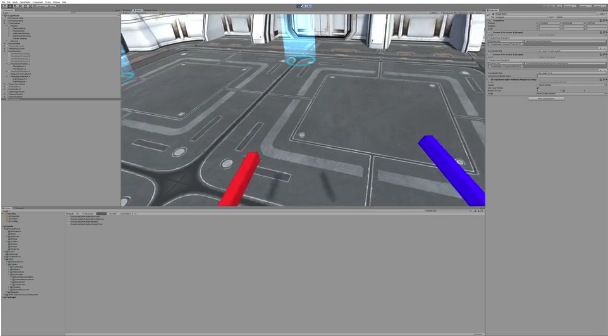
\includegraphics[width = .5\textwidth]{source/images/image47.png}
 		\captionof{figure}{\label{fig:im323} Captura previa de giro rápido con stick de control izquierdo}
	\end{center} 
\end{figure}
\begin{figure}[H]
	\begin{center}
 		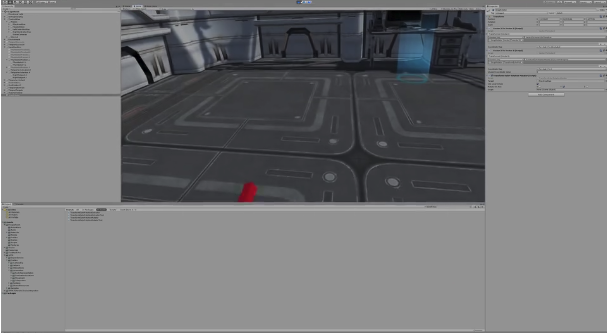
\includegraphics[width = .5\textwidth]{source/images/image71.png}
 		\captionof{figure}{\label{fig:im324}Captura posterior de giro rápido con stick de control izquierdo}
	\end{center} 
\end{figure}
Deshabilitando el objeto SnapToFloor debajo del objeto Teleporter\_.InstantPrefab en la escena.\\
Utilizando el prefabricado CollisionFader en el proyecto y arrastrándolo a la escena debajo del objeto de escena HeadsetAlias.\\
En el script CameraColorOverlay adjunto al prefabricado CollisionFader, se estableció el campo CameraValidity en el objeto de escena SceneCameras.\\
Fueron creadas dos nuevas capas llamadas FadeCamera y FadeOut. Colocando el objeto prefabricado CollisionFader en la capa FadeCamera.\\
Se colocó el objeto de la escena principal en la capa FadeOut. Se cambió la matriz de colisión para que la capa FadeCamera solo colisione con la capa FadeOut.\\
Cambiando el valor del campo ClearFlags en los scripts de la cámara bajo el GameObject de escena OVRCameraRig a color sólido y configurando el color en negro.\\

\section{Presencia e interacción de las manos}
Desde la introducción de los controles Oculus Touch para el sistema Oculus Rift y similares, la presencia de las manos ha sido la manera principal de proveer una experiencia de 
realidad virtual, los usuarios pueden encontrar manos virtuales que simulan las que poseen en realidad, esto nos ayuda a utilizar el conocimiento de los usuarios del mundo real y 
trasladarlo a el entorno virtual en lugar de tener que crear y asignar botones y crear controles complicados ya que las manos en la realidad virtual son tan importantes como en 
la realidad.\\
La implementación de manos en el sistema de realidad virtual se realizó de la manera siguiente:\\

\subsection{Agregar manos}
Se integraron los prefabricados CustomHandLeft y CustomHandRight en el proyecto y se adicionaron a  los prefabricados LeftControllerAlias y RightControllerAlias 
correspondientes en la escena.\\
Deshabilitando el script OVRGrabber en los objetos de escena CustomHandLeft y CustomHandRight.\\
Deshabilite el componente MeshRenderer para los objetos Cube en las jerarquías LeftControllerAlias y RightControllerAlias.\\
Se establecieron la capa de los objetos de escena CustomHandLeft y CustomHandRight para ignorar Raycast.\\
\begin{figure}[H]
	\begin{center}
 		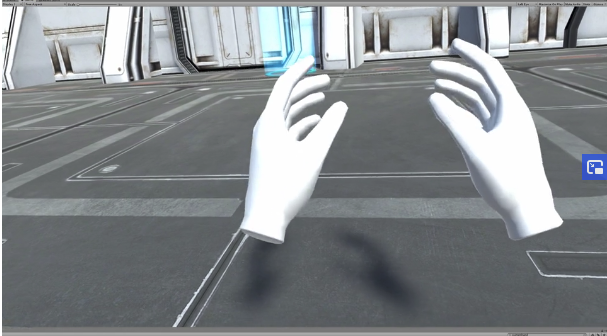
\includegraphics[width = .5\textwidth]{source/images/image74.png}
 		\captionof{figure}{\label{fig:im325}Cambio de placeholders por modelos de manos en 3D}
	\end{center} 
\end{figure}
Un método de configuración y refinamiento de la posición de las manos es utilizando el  HMD y se compara la posición de sus manos reales con la de las manos virtuales, otro método que se utilizó fue cambiar los modelos dentro del entorno mediante prueba y error, comprobando qué tan similar es la localización de los dedos conforme a la realidad comparada a lo que se ve en el entorno virtual.\\
\begin{figure}[H]
	\begin{center}
 		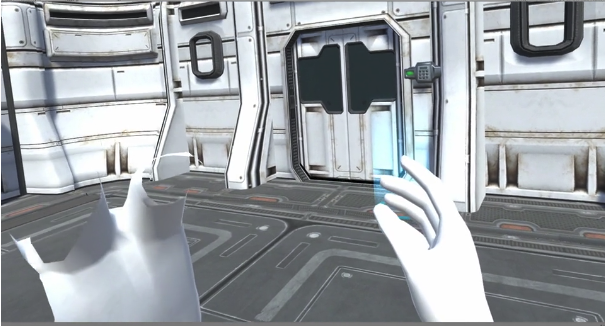
\includegraphics[width = .5\textwidth]{source/images/image48.png}
 		\captionof{figure}{\label{fig:im326}Oclusión deshabilitada para modelo de manos 3D}
	\end{center} 
\end{figure}
\begin{figure}[H]
	\begin{center}
 		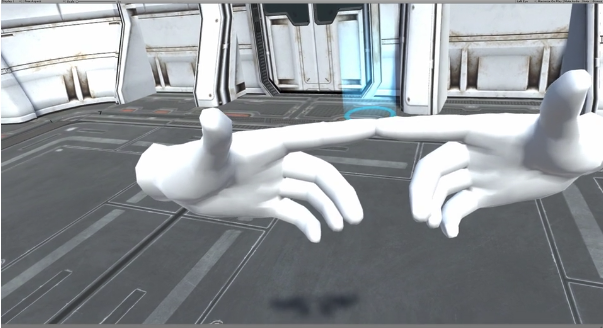
\includegraphics[width = .5\textwidth]{source/images/image23.png}
 		\captionof{figure}{\label{fig:im327}Refinado de localización de manos en el entorno virtual}
	\end{center} 
\end{figure}
Cabe mencionar que debido a la diferencia de complexión de los humanos no se puede realizar una configuración universal de estos elementos.\\
Se localizan los modelos OculusTouchRift\_.Left y OculusTouchRift\_.Right ubicados en la  escena LeftControllerAlias y RightControllerAlias respectivamente para hacer una 
representación del control en el entorno virtual, si se decide utilizarse en un futuro.\\

\subsection{Interactuando con entorno}
%Se implementa el prefab de Interactor en el proyecto y se agrega uno debajo de los prefab LeftControllerAlias ​​y RightControllerAlias ​​en la escena.
Se inhabilitó el MeshRenderer en el objeto ExampleAvatar en cada una de las jerarquías de objetos de Interactor.\\
Creando dos nuevos GameObjects para agregarlo al InputHandler y poder controlar los gatillos posteriormente y se agrega el componente en el inspector para agregar los scripts
OVRInputAxis1DAction y FloatToBoolean a cada objeto.\\
En los scripts FloatToBoolean, se establezca el campo límites positivos entre 0,75 y 1. Esto para tener una sensación de agarre conforme se va presionando el botón y no sea 
cuando ya está presionado completamente el gatillo.\\
En cada secuencia de comandos OVRInputAxis1DAction, se establezca el campo controlador en los valores L Touch y R Touch correspondientes y establezca el campo axis en 
Disparador manual primario. Se agrega componente en el inspector para agregar el script BooleanAction a cada objeto.\\
En los scripts OVRInputAxis1DAction, se agregó un nuevo objeto de acción individual en la lista de acciones individuales de ValueChanged. Agregando el GameObject principal 
y se estableció el script en FloatToBoolean/DoTransform.\\
En los scripts FloatToBoolean, se agregó un nuevo objeto de acción booleana en la lista de acciones booleanas transformadas. Agregando el GameObject principal y estableciendo 
en BooleanAction/Receive.\\
En los scripts de InteractorFacade en los prefabricados de Interactor en la escena, estableciendo el campo GrabAction en los GameObjects de script BooleanAction correspondientes.\\
Se utiliza el prefab Interactable.Primary\_.Grab.Secondary Swap en el proyecto y se agregó debajo de la jerarquía de objetos de escena y se hizo coincidir su transformación para 
los valores de transformación del objeto de escena del modelo en 3D con el cual se quiere interactuar.\\
Se deshabilitó el objeto DefaultMesh en la jerarquía Interactable.Primary\_.Grab.Secondary swap object.\\
Duplicando el objeto de escena del modelo 3D deseado y  se vuelve a pintar debajo del objeto Meshes en la jerarquía Interactable.Primary\_.Grab.Secondary\_.swap object y 
se ponga a cero los valores de transformación cuando sea necesario.\\
Se inhabilitó el objeto de escena original del modelo 3D deseado.\\
Si es necesario se ajusta la nueva transformación del modelo en 3D en los grados necesarios en el eje Y y se ajusta la transformación Interactable.Primary\_.Grab.Secondary 
swap object para ubicarse en el entorno 3D correctamente.\\

\subsection{Interacciones manuales adicionales}

Para dar una sensación de inmersión más fidedigna se integran los siguientes elementos, estos harán que la gravedad y la velocidad que es impuesta a un objeto se mantenga.\\
Se agregó el script OVRAnchorVelocityEstimator a los objetos de escena LeftHandAnchor, RightHandAnchor y CenterEyeAnchor.\\
En cada script OVRAnchorVelocityEstimator fue establecido el campo Tracked GameObject en el objeto padre del juego y el campo Relative To en el objeto de la escena TrackingSpace.\\
En el script LinkedAliasAssociationCollection adjunto al objeto de escena OVRCameraRig, establezca el campo Headset Velocity Tracker en el objeto de escena CenterEyeAnchor, 
el campo Left Controller Velocity Tracker en el objeto de escena LeftHandAnchor y el campo en el objeto de escena RightHandAnchor.\\
%Para cada prefab del interactor, se estableció el campo VelocityTracker del script InteractorFacade en el LeftControllerAlias ​​y RightControllerAlias ​​correspondientes.\\

\section{Integración de componentes del producto}
Para el integración de producto, como el mismo nombre de esta fase lo menciona los productos antes realizados, los componentes multimedia y de software finalmente se unen 
dentro del sistema.\\
